%% LGS: Lead-biased Grounding Score --- a knowledge-informed,
%% reference-free, embedding-only metric for summary quality.
%%
%% Prepared for submission to Knowledge-Based Systems (Elsevier).
%% Class: elsarticle. Bibliography style: elsarticle-num (numerical
%% citations, consistent with the in-text \cite usage).
%%
%% Highlights are supplied as a SEPARATE file (highlights.tex), as
%% required by the Elsevier submission system --- they are deliberately
%% not part of this manuscript body.

\documentclass[preprint,review,12pt]{elsarticle}

%% The amssymb package provides various useful mathematical symbols
\usepackage{amssymb}
%% The amsmath package provides various useful equation environments.
\usepackage{amsmath}

%% Layout and graphics
\usepackage[T1]{fontenc}
\usepackage[utf8]{inputenc}
\usepackage{graphicx}
\usepackage{booktabs}
\usepackage{multirow}
\usepackage{url}
\usepackage{hyperref}
\usepackage{tikz}
\usetikzlibrary{positioning,arrows.meta,calc,backgrounds}
\usepackage{pgfplots}
\pgfplotsset{compat=1.18}
\usepackage[section]{placeins}
\usepackage{float}

%% Float placement. The double-spaced review layout makes captions tall,
%% so with LaTeX's defaults the tables are deferred and pile up at the end
%% of the document. Relax the placement parameters and force every float
%% to be set before the next section begins (placeins [section] option),
%% so each table appears in the section that discusses it.
\setcounter{topnumber}{4}
\setcounter{bottomnumber}{3}
\setcounter{totalnumber}{6}
\renewcommand{\topfraction}{0.95}
\renewcommand{\bottomfraction}{0.9}
\renewcommand{\textfraction}{0.05}
\renewcommand{\floatpagefraction}{0.6}
\usepackage{algorithm}
\usepackage{algpseudocode}
%% Model tags such as \texttt{qwen2.5:7b-instruct-q4_K_M} and
%% \texttt{mxbai-embed-large} are long and, by default, unbreakable in a
%% typewriter font, which pushes lines into the margin. Allow hyphenation
%% inside \texttt and give TeX a little extra room on the final pass.
\usepackage[htt]{hyphenat}
\setlength{\emergencystretch}{3em}

\hyphenation{summ-eval embed-ding-only ref-erence-free}

%% Target Elsevier journal.
\journal{Knowledge-Based Systems}

\begin{document}

\begin{frontmatter}

\title{Lead-biased Grounding Score: injecting discourse-structural
knowledge into reference-free, cost-constrained assessment of
summary quality}

\author[wut]{Mikolaj Semeniuk}
\ead{m.semeniuk@icloud.com}

\author[wut]{Agnieszka Jastrzebska\corref{cor1}}
\ead{A.Jastrzebska@mini.pw.edu.pl}
\cortext[cor1]{Corresponding author.}

\affiliation[wut]{organization={Faculty of Mathematics and Information
                  Science, Warsaw University of Technology},
                  addressline={Koszykowa 75},
                  city={Warsaw},
                  postcode={00-662},
                  country={Poland}}

\begin{abstract}
Assessing the quality of machine-generated summaries is a decision
problem that deployed systems must solve continuously: which model
version to release, which candidate to serve, and when to block a
regression. The metrics that correlate best with human judgment are
unusable in that setting, because they require either a human-written
reference summary or a large language-model judge call per candidate.
We introduce the Lead-biased Grounding Score, a reference-free
evaluation operator that injects one explicit piece of domain
knowledge --- the journalistic convention that salient content
concentrates in the opening sentences of a news article --- as a
parametric prior over source-sentence positions, and combines it with
sentence-level grounding in a small sentence-embedding space. The
operator has a single interpretable hyperparameter and needs one
embedder forward pass per sentence: no reference, no judge, no
fine-tuned encoder. We evaluate fourteen metrics on the SummEval
benchmark under one controlled hardware budget, with wall-clock
runtime measured for every metric. Our operator attains summary-level
Spearman correlations of 0.396, 0.227, 0.156 and 0.356 on coherence,
consistency, fluency and relevance. Against thirteen published
baselines it strictly dominates six widely used metrics on the
cost--quality plane, including BERTScore, whose mean correlation it
exceeds while running ten times faster. Against trivial lead-window
controls we build in response to reviewer feedback --- keep the first
$k$ source sentences and match them lexically, no model at all --- LGS
is no longer Pareto-optimal: the cheapest lead-window control matches
or beats its raw mean correlation at roughly three orders of magnitude
lower cost. Investigating why implicates the benchmark, not only the
metric: SummEval's human ratings are substantially confounded with
how much a candidate copies verbatim from the source, and a
zero-parameter bigram copy-rate counter outranks eleven of the
fourteen published metrics in our pool on this axis. Once that
confound is partialled out, LGS is no longer statistically
distinguishable from the cheapest lead-window control, though it ties
BERTScore. Re-running
the entire selection procedure inside a cluster bootstrap further shows
that the knowledge prior is worth switching on --- the no-prior setting
is selected in under 1\% of resamples --- but that its exponent is not
identifiable at benchmark scale: the reported value is selected in 18\%
of resamples, and an unchanged backbone scored on two draws of the same
50 articles agrees with itself on the exponent only 44\% of the time.
We therefore present the prior as a design element carrying an
obligatory, and demonstrably underdetermined, calibration step.
\end{abstract}

\begin{keyword}
Summarization quality assessment \sep reference-free evaluation \sep
knowledge-informed prior \sep sentence embeddings \sep
cost-aware decision support \sep hyperparameter calibration
\end{keyword}

\end{frontmatter}

% ------------------------------------------------------------------
\section{Introduction}
\label{sec:intro}

Every organisation that operates a summarisation service has to answer
the same question many times a day: \emph{is this summary good enough?}
The question arises when a new model checkpoint is proposed for
release, when several decoding configurations compete for the same
request, when a nightly regression suite must decide whether a change
degraded output quality, and when a reinforcement-learning loop needs a
scalar reward for a freshly sampled candidate. In all of these
situations the answer is consumed by an automated decision procedure,
not by a human reader, and it must be produced quickly, deterministically,
and without any artefact that a production pipeline does not have.

The evaluation metrics that agree best with human judgment fail exactly
this test. Reference-based metrics, including
BLEU~\cite{papineni2002bleu}, ROUGE-L~\cite{lin2004rouge},
METEOR~\cite{banerjee2005meteor}, ChrF~\cite{popovic2015chrf},
BERTScore~\cite{zhang2020bertscore},
MoverScore~\cite{zhao2019moverscore},
BARTScore~\cite{yuan2021bartscore} and SMART~\cite{amplayo2022smart},
all presuppose a human-written reference summary --- a precondition
that production inputs never satisfy, because the candidate is the only
summary in the system. The two strongest \emph{reference-free}
contenders on the \textsc{SummEval}~\cite{fabbri2021summeval}
benchmark avoid that dependency but replace it with an inference cost
that dominates the engineering budget: UniEval requires a fine-tuned
T5-large pass per (article, candidate, dimension)
tuple~\cite{zhong2022unieval}, and G-Eval queries a large
language-model judge with a chain-of-thought prompt and aggregates over
multiple sampled generations~\cite{liu2023geval}. Recent surveys of
reference-free text-generation metrics~\cite{ito2025reffree} and of
the LLM-as-a-judge paradigm~\cite{gu2024judgesurvey} document the same
tension: judge-based evaluation buys correlation with human raters at
the price of latency, monetary cost, non-determinism and
reproducibility.

There is, however, a resource that deployed summarisation pipelines do
possess and that current metrics leave unused: \emph{explicit knowledge
about how source documents are structured}. News writing follows the
inverted-pyramid convention, in which the most newsworthy material is
placed in the opening sentences; the resulting \emph{lead bias} of
news corpora is one of the best-documented regularities in the
summarisation literature~\cite{kedzie2018content,grusky2018newsroom}.
This knowledge costs no extra model forward pass at inference time ---
applying it is a closed-form arithmetic reweighting of a similarity
already computed, not an additional model, annotation or retrieval
step --- and it is exactly the kind of
structural domain regularity that a knowledge-informed system should
encode explicitly rather than hope a learned representation will
rediscover.

\subsection{Contributions}
This paper makes the following contributions.

\begin{enumerate}
\item \textbf{A knowledge-informed evaluation operator.} We define the
Lead-biased Grounding Score (LGS), which combines sentence-level
grounding of the candidate in the source with an explicit,
one-parameter prior over source-sentence position that encodes
discourse-structural knowledge about news documents
(Section~\ref{sec:method}). The operator is reference-free,
interpretable --- every candidate sentence is anchored to one
identifiable source sentence --- and runs at one small-embedder
forward pass per sentence, with no judge call and no fine-tuned
encoder.

\item \textbf{A cost-controlled benchmark of fourteen metrics.} We
reproduce thirteen published metrics plus LGS on \textsc{SummEval}
under one hardware budget and one runtime harness, and report
wall-clock cost per sample alongside correlation for every metric
(Section~\ref{sec:cost}). To our knowledge, no prior meta-evaluation
of summarisation metrics reports measured deployment cost and
correlation on the same axis for a baseline pool of this size.

\item \textbf{A Pareto analysis of the cost--quality plane, including
trivial lead-window controls, and the extractiveness confound this
analysis exposes.} Among the fourteen published metrics, LGS strictly
dominates six widely deployed metrics, among them BERTScore, which it
exceeds in mean summary-level Spearman $\rho$ while running roughly
ten times faster, and the LLM-judge metric in our reproduction is
itself dominated by the fine-tuned-encoder metric. But when the pool
is extended with reference-free lead-window controls --- keep the
first $k$ source sentences, match with ROUGE-L, no model --- LGS is
\emph{not} Pareto-optimal: the cheapest control matches or exceeds its
raw mean correlation at roughly $950\times$ lower cost
(Section~\ref{sec:pareto}). We trace this to a confound: SummEval's
human ratings substantially reward verbatim copying from the source,
and a parameter-free copy-rate counter alone outranks eleven of the
fourteen published metrics on mean correlation. Controlling for this
confound, LGS is not statistically distinguishable from the cheapest
lead-window control and ties BERTScore (Section~\ref{sec:confound}).
We report this as a limitation of the metric and, more importantly, of
the benchmark axis itself.

\item \textbf{A measurement of how much of a tuned structural prior is
signal and how much is the luck of the development draw.} Metric
papers report the selected hyperparameter as a number; we instead
re-run the \emph{entire selection procedure} on every cluster-bootstrap
resample and report the resulting distribution over grid values
(Section~\ref{sec:lambda-identifiability}). Two facts follow. Switching
the prior on is robust: $\lambda{=}0$ is selected in $0.7\%$ of
development resamples and $0.3\%$ of test resamples. Which exponent to
switch it to is not: the reported $\lambda^{*}{=}0.5$ is selected in
$17.8\%$ of resamples, and a fixed backbone compared against itself on
two independent draws of the same 50 articles agrees on the exponent
only $43.5\%$ of the time. We therefore present LGS as a design plus an
obligatory calibration protocol (Section~\ref{sec:methodology}) whose
output is a usable interval rather than a reproducible point, and we
report the width of that interval instead of suppressing it.

\item \textbf{A reproducible artefact.} The full pipeline --- all
fourteen metrics, the calibration sweep, the backbone ablation and
every table and figure in this paper --- is released as open-source
code with a single-command reproduction path at
\url{https://github.com/mikolajsemeniuk/llmbench}.
\end{enumerate}

We are explicit from the outset about what is \emph{not} claimed. LGS
does not attain the highest correlation with human judgment in our
pool: UniEval does, and we report that plainly. Nor is LGS
Pareto-optimal once trivial lead-window controls enter the pool: a
four-line lexical heuristic matches or beats it on raw mean
correlation at far lower cost, and the two are not statistically
distinguishable once the benchmark's extractiveness confound is
controlled for. The claim we defend is narrower: among metrics that
perform any learned or embedding-based computation, LGS occupies a
cost--quality point that none of them dominates, and it is the
cheapest metric in the pool that ties BERTScore's confound-controlled
correlation.

\subsection{Structure of the paper}
Section~\ref{sec:related} surveys reference-based and reference-free
metrics, organises them by the knowledge source they consume, and
states the research gap. Section~\ref{sec:method} defines LGS,
gives its algorithm and computational complexity, and motivates each
design choice. Section~\ref{sec:methodology} presents the calibration
protocol for the knowledge prior and explains why it is a necessary
rather than a decorative step. Section~\ref{sec:experiments} describes
the experimental protocol. Section~\ref{sec:cost} reports the
cost--quality analysis, including the Pareto frontier.
Section~\ref{sec:results} reports correlations with human judgment
together with paired-bootstrap significance tests, the prior sweep, the
backbone ablation, and the cross-backbone calibration result.
Section~\ref{sec:discussion} discusses deployment, limitations and
threats to validity, and Section~\ref{sec:conclusion} concludes.

% ------------------------------------------------------------------
\section{Related Work and Research Gap}
\label{sec:related}

\subsection{Reference-based metrics}
The longest-standing family of summarisation metrics is
reference-based: a candidate summary is compared against one or
more human-written reference summaries.
N-gram precision and recall metrics
(BLEU~\cite{papineni2002bleu}, ROUGE-L~\cite{lin2004rouge},
METEOR~\cite{banerjee2005meteor}, ChrF~\cite{popovic2015chrf})
operate on surface-form overlap. Their well-documented blind spot
is that paraphrases of equivalent content score low simply because
the surface forms differ, which is precisely the regime
abstractive summarisation operates in.
Contextual-embedding metrics replace surface overlap with cosine
similarity in a learned representation space derived from
Transformer encoders~\cite{vaswani2017attention,devlin2019bert}:
BERTScore~\cite{zhang2020bertscore} matches token embeddings
greedily, MoverScore~\cite{zhao2019moverscore} solves a
transportation problem over them, BARTScore~\cite{yuan2021bartscore}
re-uses the encoder--decoder log-likelihood under a pretrained
generation model based on BART~\cite{lewis2020bart}, and
SMART~\cite{amplayo2022smart} extends the matching to sentence
units. A parallel line of work in machine translation evaluation
learns metric weights directly against human judgments
(BLEURT~\cite{sellam2020bleurt}, COMET~\cite{rei2020comet}), and
on the summarisation side a related family targets faithfulness
specifically (FactCC~\cite{kryscinski2020factcc} for factual
consistency classification, SummaC~\cite{laban2022summac} for
NLI-based inconsistency detection). They alleviate the paraphrase
problem but inherit the same structural dependence on the
reference: the score is a function of (reference, candidate)
pairs and is undefined when no reference exists.

\subsection{Reference-free and source-based metrics}
A smaller body of work scores candidates against the \emph{source}
article rather than against a human reference, removing the
deployment dependency on hand-written summaries; a recent survey
maps this family across generation tasks~\cite{ito2025reffree}.
G-Eval~\cite{liu2023geval} prompts a large language
model~\cite{brown2020gpt3} with a
chain-of-thought rubric~\cite{wei2022cot} to score each
(source, candidate) pair on
the relevant dimension. It obtains the strongest published
correlation on \textsc{SummEval}'s consistency dimension among
published metrics, but at a substantial cost: one or more LLM-judge
calls per (article, candidate, dimension) tuple, with sampled
decoding requiring repeated calls per pair to absorb LLM-judge
variance (the original paper averages 20 GPT-4 samples). Surveys of
the judge paradigm document the accompanying issues of prompt
sensitivity, length bias, non-determinism and dependence on
proprietary, frequently-updated
endpoints~\cite{gu2024judgesurvey}, and a growing line of work
explicitly targets cheaper substitutes for judge calls in
evaluation~\cite{balamurali2025nli}. The metric is therefore
inappropriate for deployment scenarios that require deterministic,
low-latency, high-throughput scoring.
UniEval~\cite{zhong2022unieval} is a hybrid: a fine-tuned T5-large
encoder~\cite{raffel2020t5} is queried with a Boolean question
(``Is this summary \{coherent, consistent, fluent, relevant\}?'')
and the score is the posterior probability of ``Yes''. UniEval
sidesteps the LLM-judge cost but still requires a fine-tuned
encoder per dimension and a forward pass per
(article, candidate, dimension) tuple.
GPTScore~\cite{fu2023gptscore} re-uses a pretrained language model
to compute a per-token log-likelihood of the candidate conditioned
on the source, requiring a single forward pass per pair but
inheriting the model's calibration as the score's calibration.

A pre-LLM family of reference-free, source-based metrics is the
closest prior art to LGS and must be positioned explicitly.
SUPERT~\cite{gao2020supert} builds a \emph{pseudo-reference} by
extracting salient source sentences and then scores the candidate
against that pseudo-reference with contextual-embedding similarity;
ESTIME~\cite{vasilyev2021estime} uses BERT embeddings to flag
points of semantic mismatch between summary and source directly,
without an intermediate reference; BLANC~\cite{vasilyev2020blanc}
measures how much a summary improves a masked-language model's
ability to reconstruct held-out source tokens; and
SummaQA~\cite{scialom2019summaqa} checks whether a QA model can
answer source-derived cloze questions using only the summary.
SUPERT and ESTIME are mechanistically the closest antecedents to
LGS: SUPERT already performs reference-free, salience-sensitive,
embedding-based scoring against the source, and ESTIME already
performs embedding-level grounding checks between summary and
source without an intermediate reference. LGS differs from this
family in two specific ways rather than in kind: (a) it grounds
each \emph{candidate sentence} directly against raw source sentences
via mean-of-max cosine, instead of comparing against an intermediate
pseudo-reference (SUPERT) or an auxiliary masked-LM/QA task (BLANC,
SummaQA); and (b) it encodes positional lead bias as an explicit,
tunable multiplicative prior inside the scoring function, rather than
leaving position implicit in an extraction step. The contribution
claimed below is this specific combination --- direct sentence-level
grounding plus an explicit, calibrated lead-position prior, evaluated
jointly against deployment cost --- not the introduction of
reference-free source-grounded evaluation as a category, which this
family already established.

\subsection{The closest control: whole-text embedding cosine}
The simplest reference-free embedding baseline is a single cosine
similarity between the embedding of the entire source and the
embedding of the entire candidate, computed with the same
sentence-embedder used by the metric under test. We call this
baseline \textsc{EmbedScorer}. Two properties make it
ideal for like-for-like comparison with LGS. First, it shares the
embedder backbone, so any difference between the two metrics is
attributable to the architectural choices of LGS --- sentence-level
grounding via $\max_i$ on the source side, mean aggregation on the
candidate side, and the position prior $w(i)$ --- and not to a
stronger or weaker embedding model.
Second, both metrics are reference-free; the comparison isolates
the architectural contribution from the orthogonal question of
whether reference-based metrics are stronger than reference-free
ones in general. We return to the \textsc{EmbedScorer}-vs-LGS gap as
the controlled ablation of the knowledge component in
Section~\ref{sec:results}.

\subsection{Research gap}
\label{sec:gap}
Table~\ref{tab:families} organises the metric pool \emph{benchmarked in
this paper} by the knowledge sources each metric consumes at inference
time; SUPERT, BLANC, SummaQA and ESTIME are discussed above but are
not run in our controlled-budget harness and so are not rows of this
table. Within the benchmarked pool, no metric consumes \emph{a priori
knowledge about the structure of the source document} as an explicit,
inspectable scoring component, even though such knowledge costs no
extra forward pass to apply and is one of the most robust regularities
in the news domain that the dominant benchmarks are built on. SUPERT is
the closest published exception, and it encodes source structure only
implicitly, through which sentences its extractive pseudo-reference
step happens to select, not as a separately calibrated parameter.

Prior systems do exploit lead bias, but only \emph{implicitly} and
only on the generation side: the lead-3 extractive baseline is a
standing strong competitor on CNN/DailyMail, and pretrained
encoder--decoder summarisers absorb the same prior through their
training
distribution~\cite{liu2019bertsum,zhang2020pegasus,see2017pointer}.
On the \emph{evaluation} side, published reference-free metrics
either leave the prior implicit (SUPERT's pseudo-reference
extraction) or do not use it at all. LGS extends this line by making
the structural prior an explicit, inspectable,
single-parameter component of the scoring function --- and, because
it is explicit, a component that can be ablated, swept, and shown to
be necessary or not, which an implicitly-absorbed prior cannot.

A second gap concerns how metric papers are evaluated. Published
meta-evaluations report correlation with human judgment but not
measured deployment cost on the same axis for a comparable-sized
baseline pool; MetaMetrics~\cite{metametrics2024}, for instance,
benchmarks thirteen summarisation metrics but reports only a
parameter count for one reward-model variant, not runtime, and only
for that variant. Without a cost axis
one cannot tell whether a metric is a sensible deployment choice or
merely a strong one, and one cannot detect metrics that are dominated
--- slower \emph{and} weaker than an available alternative.
Section~\ref{sec:cost} supplies that axis under a single controlled
budget and shows that domination is common in the current pool.

Each column below is defined independently of LGS, so the table can
be read without circularity: \emph{Ref.} is whether the metric's score
is a function of a human-written reference summary (undefined without
one); \emph{Src.} is whether it reads the source article at all;
\emph{Model} is whether scoring requires a pretrained or fine-tuned
neural network (a lexical metric needs none); \emph{Judge} is whether
an autoregressive LLM is prompted to produce the rating directly,
rather than a fixed scoring function consuming a representation;
\emph{Prior} is whether document-position information is an explicit,
separately inspectable and tunable input to the scoring function, as
opposed to being absorbed implicitly by a learned representation or by
an upstream extraction step (Section~\ref{sec:gap} discusses SUPERT,
the one published metric that uses source structure implicitly).
LGS's own row follows directly from these definitions rather than
being asserted: it has no Ref.\ tick because Equation~\ref{eq:lgs}
never receives a reference summary as input, and no Judge tick because
scoring is a fixed cosine-and-argmax computation with no LLM call
anywhere in it --- the same reason G-Eval is the only Judge row and
UniEval, despite consuming both source and reference, is not, since
its score is a fine-tuned encoder's posterior rather than a
prompted judgment. A blank cell means the column's resource is absent
from that metric's inputs, not merely unreported.

\begin{table*}[t]
\centering
\caption{The metric pool organised by the knowledge sources consumed
at inference time; see the paragraph above for how each column is
defined and how to read a blank cell.}
\label{tab:families}
\footnotesize
\begin{tabular}{@{}p{0.235\linewidth} p{0.185\linewidth} ccccc@{}}
\toprule
\textbf{Metric} & \textbf{Family} & \textbf{Ref.} & \textbf{Src.}
& \textbf{Model} & \textbf{Judge} & \textbf{Prior} \\
\midrule
BLEU, ROUGE-L, ChrF, METEOR & lexical overlap    & \checkmark & --- & --- & --- & --- \\
SMART-String                & lexical, sentence  & \checkmark & --- & --- & --- & --- \\
\textsc{EmbedScorer}        & embedding, doc.    & \checkmark & --- & \checkmark & --- & --- \\
SMART-Model                 & embedding, sent.   & \checkmark & --- & \checkmark & --- & --- \\
BERTScore                   & embedding, token   & \checkmark & --- & \checkmark & --- & --- \\
MoverScore                  & embedding, transp. & \checkmark & --- & \checkmark & --- & --- \\
BARTScore, GPTScore         & likelihood         & \checkmark & --- & \checkmark & --- & --- \\
UniEval                     & fine-tuned QA      & \checkmark & \checkmark & \checkmark & --- & --- \\
G-Eval                      & LLM judge          & ---        & \checkmark & \checkmark & \checkmark & --- \\
\textbf{LGS (this work)}    & embedding, sent.   & ---        & \checkmark & \checkmark & --- & \checkmark \\
\bottomrule
\end{tabular}
\end{table*}

% ------------------------------------------------------------------
\section{The Lead-biased Grounding Score}
\label{sec:method}

\subsection{Notation}
Table~\ref{tab:notation} collects the symbols used in the definition
below and reused throughout Sections~\ref{sec:method}--\ref{sec:results}.

\begin{table}[t]
\centering
\caption{Notation used to define LGS and its calibration protocol.}
\label{tab:notation}
\small
\begin{tabular}{@{}ll@{}}
\toprule
Symbol & Meaning \\
\midrule
$D$ & Source document \\
$C$ & Candidate summary \\
$n$, $m$ & Number of source / candidate sentences \\
$s_i$, $c_j$ & $i$-th source sentence, $j$-th candidate sentence \\
$\mathrm{emb}(\cdot)$ & Sentence embedder (Sentence-BERT family) \\
$\cos(\cdot,\cdot)$ & Cosine similarity between two embeddings \\
$w(i)$ & Source-position (lead-bias) prior weight \\
$\lambda$ & Lead-bias exponent, the metric's one hyperparameter \\
$\lambda^{\star}$ & Dev-selected value of $\lambda$ \\
$\hat\lambda$ & Dev-argmax $\lambda$ for a single dimension (Table~\ref{tab:lambdadim}) \\
$\rho$ & Spearman rank correlation with human ratings \\
$\bar\rho$ & Mean $\rho$ across the four \textsc{SummEval} dimensions \\
$\bar\rho_{\mathrm{part}}$ & $\bar\rho$ with copy rate partialled out (Section~\ref{sec:confound-analysis}) \\
\bottomrule
\end{tabular}
\end{table}

\subsection{Definition}
Let $D$ be a source document split into $n$ sentences
$s_0,\dots,s_{n-1}$ and let $C$ be a candidate summary split into
$m$ sentences $c_0,\dots,c_{m-1}$. Let $\mathrm{emb}(\cdot)$ be a
sentence embedder of the Sentence-BERT
family~\cite{reimers2019sbert}
(in the empirical part, we use \texttt{nomic-embed-text}~\cite{nussbaum2024nomic}
served via Ollama, see Section~\ref{sec:experiments}). The Lead-biased
Grounding Score is defined as
\begin{equation}
\label{eq:lgs}
\mathrm{LGS}(D,C) \;=\; \frac{1}{m}\sum_{j=0}^{m-1}
\;\max_{0\le i<n}\; w(i)\cdot \cos\!\bigl(\mathrm{emb}(c_j),
\mathrm{emb}(s_i)\bigr),
\end{equation}
where the source-position prior is
\begin{equation}
\label{eq:wprior}
w(i) \;=\; \exp\!\bigl(-\lambda \cdot i / n\bigr),
\end{equation}
$i=0$ denotes the lead sentence, and $\lambda \ge 0$ is the only
hyperparameter. $\lambda=0$ disables the prior and reduces LGS to
position-agnostic mean-of-max recall.
Figure~\ref{fig:lgs-schematic} illustrates the operator
graphically.

\begin{figure*}[t]
\centering
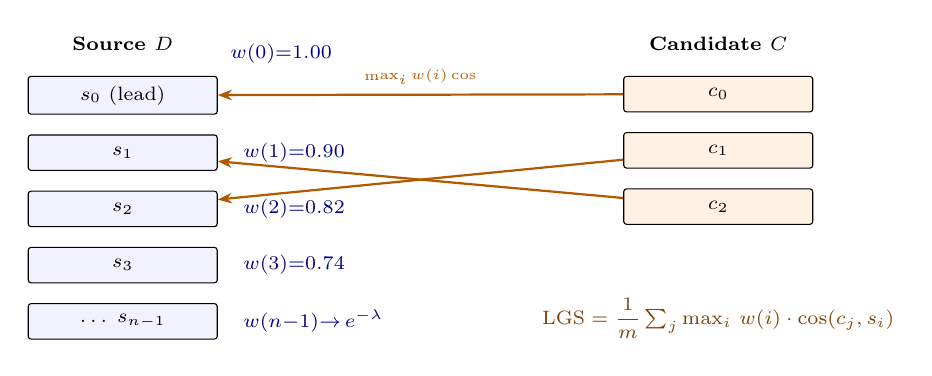
\begin{tikzpicture}[
  node distance=2.5mm,
  src/.style={draw, rounded corners=1pt, minimum width=24mm,
              minimum height=4.5mm, font=\scriptsize, align=center,
              fill=blue!5},
  cand/.style={draw, rounded corners=1pt, minimum width=24mm,
               minimum height=4.5mm, font=\scriptsize, align=center,
               fill=orange!10},
  pick/.style={-{Stealth[length=1.8mm]}, thick, orange!70!black},
  weight/.style={font=\scriptsize\itshape, anchor=west,
                 text=blue!50!black},
  hdr/.style={font=\scriptsize\bfseries, align=center}
]
  % Source column
  \node[hdr] (srchdr) {Source $D$};
  \node[src, below=2mm of srchdr] (s0) {$s_0$ (lead)};
  \node[src, below=of s0] (s1) {$s_1$};
  \node[src, below=of s1] (s2) {$s_2$};
  \node[src, below=of s2] (s3) {$s_3$};
  \node[src, below=of s3] (s4) {$\dots\;s_{n-1}$};
  % Weights
  \node[weight, above right=0.5mm of s0] {$w(0){=}1.00$};
  \node[weight, right=2mm of s1] {$w(1){=}0.90$};
  \node[weight, right=2mm of s2] {$w(2){=}0.82$};
  \node[weight, right=2mm of s3] {$w(3){=}0.74$};
  \node[weight, right=2mm of s4] {$w(n{-}1){\to}\,e^{-\lambda}$};

  % Candidate column
  \node[hdr, right=58mm of srchdr] (candhdr) {Candidate $C$};
  \node[cand, below=2mm of candhdr] (c0) {$c_0$};
  \node[cand, below=of c0] (c1) {$c_1$};
  \node[cand, below=of c1] (c2) {$c_2$};

  % Argmax arrows (illustrative)
  \draw[pick] (c0) -- (s0)
    node[midway, above, font=\tiny\itshape, sloped] {$\max_i w(i)\cos$};
  \draw[pick] (c1) -- (s2);
  \draw[pick] (c2) -- (s1);

  % Aggregation note
  \node[font=\scriptsize, below=8mm of c2, anchor=north,
        align=center, text=orange!50!black] (agg)
    {$\mathrm{LGS}=\dfrac{1}{m}\sum_{j} \max_i\, w(i)\cdot\cos(c_j, s_i)$};
\end{tikzpicture}
\caption{LGS operator. For each candidate sentence $c_j$, the
metric finds the source sentence $s_i$ that maximises the
position-weighted cosine similarity $w(i)\cdot\cos(c_j, s_i)$,
where $w(i)=\exp(-\lambda i/n)$ is an exponential prior favouring
the lead. The score is the mean of these per-candidate maxima.
Orange arrows indicate illustrative argmax matches.}
\label{fig:lgs-schematic}
\end{figure*}

\subsection{Algorithm and computational complexity}
\label{sec:complexity}
Algorithm~\ref{alg:lgs} states the procedure. Every step is
deterministic given the embedder, and the argmax index recorded in
line~\ref{line:argmax} is the interpretability handle: it names the
source sentence that the operator considers to be the evidence for
each candidate sentence, so a low score can always be traced to the
specific summary sentences that failed to find an anchor.

\begin{algorithm}[t]
\caption{Lead-biased Grounding Score}
\label{alg:lgs}
\begin{algorithmic}[1]
\Require source document $D$, candidate summary $C$, exponent
$\lambda \ge 0$, sentence embedder $\mathrm{emb}(\cdot)$
\Ensure score in $[0, 1]$ (negative cosine similarities are clamped
to 0), plus per-sentence evidence anchors
\State $(s_0,\dots,s_{n-1}) \gets \textsc{SplitSentences}(D)$
\State $(c_0,\dots,c_{m-1}) \gets \textsc{SplitSentences}(C)$
\State $E^{s}_{i} \gets \mathrm{emb}(s_i)$ for $i = 0,\dots,n-1$
  \Comment{cached per source document}
\State $E^{c}_{j} \gets \mathrm{emb}(c_j)$ for $j = 0,\dots,m-1$
\For{$i \gets 0$ \textbf{to} $n-1$}
  \State $w_i \gets \exp(-\lambda \cdot i / n)$
    \Comment{structural prior, length-normalised}
\EndFor
\State $\mathrm{total} \gets 0$
\For{$j \gets 0$ \textbf{to} $m-1$}
  \State $a_j \gets \arg\max_{0 \le i < n}\; w_i \cdot
         \cos(E^{c}_{j}, E^{s}_{i})$ \label{line:argmax}
    \Comment{evidence anchor for $c_j$}
  \State $\mathrm{total} \gets \mathrm{total} +
         w_{a_j}\cdot\cos(E^{c}_{j}, E^{s}_{a_j})$
\EndFor
\State \Return $\max(0,\ \mathrm{total} / m)$, $(a_0,\dots,a_{m-1})$
\end{algorithmic}
\end{algorithm}

Let $d$ be the embedding dimension and let $T$ be the cost of one
embedder forward pass. Embedding costs $\mathcal{O}\bigl((n+m)\,T\bigr)$
and dominates in practice; the similarity stage costs
$\mathcal{O}(nmd)$ floating-point operations and the prior costs
$\mathcal{O}(n)$. Memory is $\mathcal{O}\bigl((n+m)d\bigr)$, since the
$n \times m$ similarity matrix need never be materialised --- the
maximum over $i$ can be accumulated in a single pass per candidate
sentence.

Two properties matter for deployment. First, source embeddings depend
only on $D$, so when $K$ candidates are scored against the same
article --- the standard situation in model selection and in
reinforcement-learning rollouts --- the source cost is paid once and
amortised, giving $\mathcal{O}\bigl((n + Km)T\bigr)$ instead of
$\mathcal{O}\bigl(K(n+m)T\bigr)$. Second, the exponent $\lambda$
enters only through the weight vector $w$, so a full sweep over a
$\lambda$-grid of size $G$ reuses one set of embeddings and costs
$\mathcal{O}(Gnmd)$ additional arithmetic with no additional forward
passes. Calibration (Section~\ref{sec:methodology}) is therefore
essentially free relative to scoring, which is what makes an
obligatory per-deployment sweep a realistic requirement rather than a
burden.

For contrast, a judge-based metric costs one or more autoregressive
decodes per (article, candidate, dimension) tuple, with the decode
length itself dependent on the rubric; a fine-tuned-encoder metric
costs one encoder pass per tuple, and thus scales linearly in the
number of quality dimensions, which LGS does not.

\subsection{Worked example}
To make the operator concrete, consider a stylised article with
$n{=}5$ source sentences --- $s_0$: ``Apple announced a new
iPhone at its September event.''; $s_1$: ``The phone features an
improved camera system.''; $s_2$: ``Tim Cook presented the
keynote in Cupertino.''; $s_3$: ``Pre-orders begin Friday.'';
$s_4$: ``Stock rose 3\% after the announcement.'' --- and a
candidate summary with $m{=}2$ sentences --- $c_0$: ``Apple
unveiled a new iPhone.''; $c_1$: ``Pricing starts at \$999.''.
Suppose, for illustration purposes, that the cosine similarity matrix
between the candidate sentence embeddings and the source
sentence embeddings is
\[
\bigl[\cos(c_j, s_i)\bigr]_{j,i} =
\begin{pmatrix}
0.91 & 0.41 & 0.52 & 0.18 & 0.34 \\
0.22 & 0.31 & 0.15 & 0.78 & 0.42
\end{pmatrix}.
\]
At $\lambda{=}0.5$ the position prior takes values
$w(0){\approx}1.00$, $w(1){\approx}0.90$, $w(2){\approx}0.82$,
$w(3){\approx}0.74$, $w(4){\approx}0.67$. For $c_0$ the
position-weighted argmax is $s_0$ (weighted similarity
$1.00{\cdot}0.91{=}0.91$); for $c_1$ it is $s_3$
($0.74{\cdot}0.78{=}0.58$). The score is the mean of these
two per-candidate maxima, $\mathrm{LGS}{=}(0.91{+}0.58)/2{=}0.745$.

A hallucinated $c_1$ that is unrelated to the source --- say,
``Tim Cook resigned as CEO.'' with (assumed for illustration purposes) cosine row
$(0.18, 0.09, 0.55, 0.11, 0.21)$ --- yields position-weighted
maximum $0.82{\cdot}0.55{=}0.451$ on $s_2$, and the score drops
to $(0.91{+}0.45)/2{=}0.680$. The metric's sensitivity to
ungrounded content is structurally tied to the candidate-side
mean: with candidate length $m$, a single ungrounded sentence
removes approximately $1/m$ of the score's mass.

\subsection{Design rationale}
\paragraph{Sentence-level grounding}
A candidate sentence is \emph{grounded} when some source sentence
semantically supports it. The LGS metric (Eq.~\ref{eq:lgs}) implements
this by taking,
for each candidate sentence $c_j$, the maximum cosine similarity
to any source sentence under the position prior, and then
aggregating across the candidate with a mean. The asymmetry is
deliberate: $\max_i$ on the source side is a localised signal
(``does this candidate sentence have \emph{any} anchor in the
source?''); $\mathrm{mean}_j$ on the candidate side is a
hallucination-sensitive aggregate (a single ungrounded
candidate sentence depresses the score by $1/m$, where $m$ is the
candidate length, rather than being washed out by an averaging
operator on both sides). We compared this asymmetric mean-of-max
formulation empirically against alternative aggregations during
the calibration phase --- low-percentile recall, top-$k$ recall,
candidate-side coverage exponent --- and report the negative
results in Appendix~\ref{app:extension-log}; none lifted
the development-set mean Spearman over the mean-of-max baseline.

\paragraph{Which knowledge is injected, and why exponentially}
News summarisation corpora --- and CNN/DailyMail in
particular~\cite{hermann2015cnndm,see2017pointer}, the source of
all \textsc{SummEval} articles ---
exhibit well-documented \emph{lead
bias}~\cite{kedzie2018content,grusky2018newsroom}: salient
information is disproportionately concentrated in the opening
sentences of the article, a pattern reinforced by the
inverted-pyramid convention of journalistic writing. This is the
single piece of a priori domain knowledge that LGS encodes, and it
enters the scoring function as a multiplicative source-side prior
$w(i)=\exp(-\lambda i / n)$ rather than being left for the embedder
to infer.
The exponential family is chosen for three reasons. First,
parsimony: it is the simplest one-parameter decay shape that
interpolates between a uniform prior ($\lambda{=}0$) and a
near-step prior ($\lambda \to \infty$) without introducing a
discontinuity. Second, scale-invariance: normalising the position
$i$ by the document length $n$ makes the prior behave
consistently across short and long articles, removing the need
for a length-dependent tuning of $\lambda$. Third, multiplicative
interaction: the prior reweights the cosine similarity \emph{before}
the $\max_i$ operator, so it can move which source sentence wins
the argmax for a given candidate; an additive prior would only
shift scores uniformly without affecting the matching structure.
The choice of an explicit prior over an implicit one is what makes
the knowledge component \emph{auditable}: $\lambda{=}0$ removes it
exactly, so its contribution can be measured rather than asserted
(Section~\ref{sec:ablation-lambda}).

\paragraph{Why a single hyperparameter}
The canonical LGS has exactly one tunable scalar, $\lambda$.
Possible alternative formulations of this metric can be richer: a precision side
mirroring BERTScore's F-measure structure, a candidate-side
coverage exponent that rewarded using more distinct source
anchors, a within-summary diversity penalty, and a top-$k$ source
aggregation. We tested each of these alternatives on the same held-out
development split (Section~\ref{sec:methodology}) and rejected them for
failing to
lift the development-set mean Spearman $\rho$ over the no-prior
baseline. The rejected components and their negative numbers are
reported in Appendix~\ref{app:extension-log}. The
single-hyperparameter design is the one we propose.
A beneficial corollary of this discipline is that the calibration
protocol has a small, well-defined search space (one scalar over a 1-D
grid), which --- combined with the embedding reuse noted in
Section~\ref{sec:complexity} --- makes recalibration cheap enough to
be mandatory.

\paragraph{Relation to BERTScore}
The closest already-existing metric is BERTScore~\cite{zhang2020bertscore}, which also computes a
mean-of-max over cosine similarities between embedded units.
However, there are three essential operational differences between LGS and BERTScore. First, BERTScore matches \emph{tokens} (BPE or wordpiece)
under a contextual encoder. In contrast, LGS matches \emph{sentences} under a
sentence encoder. The unit choice changes the semantic
granularity: a token-level $\max_i$ rewards lexical or stylistic
overlap, while a sentence-level $\max_i$ rewards proposition-level
grounding and is structurally less sensitive to surface paraphrase.
Second, BERTScore is reference-based: one side of every $\max$ is
a human reference summary. LGS is reference-free: one side is the
\emph{source article}, removing the deployment dependency on
human-written summaries (Section~\ref{sec:related}). The
cost--quality implications differ accordingly: BERTScore's
correlation gain over n-gram metrics buys nothing in
deployments where no reference exists. Third, neither BERTScore
nor any other published mean-of-max metric uses a source-position
prior. The lead-bias prior $w(i)$ in LGS is the architectural
ingredient that distinguishes it from a structurally simpler
``sentence-BERTScore against the source'' baseline; the
\textsc{EmbedScorer}-vs-LGS comparison in
Section~\ref{sec:results} is the controlled experiment that
isolates this contribution.

% ------------------------------------------------------------------
\section{Calibrating the Knowledge Prior}
\label{sec:methodology}

\subsection{Why calibration is a first-class step}
A structural prior is a statement about the source documents, but it
acts inside a learned representation space, and the two interact. Two
separate findings make the sweep obligatory rather than decorative.

First, the point estimate of the optimum differs across backbones:
with \texttt{nomic-embed-text} the development-set optimum is
$\lambda^{*}\!=\!0.5$, with \texttt{bge-m3}~\cite{chen2024bgem3} it is
$\lambda^{*}\!=\!0.25$, and applying the nomic-tuned value to
\texttt{bge-m3} \emph{underperforms} the no-prior baseline
(Section~\ref{sec:ablation-lead-bge}).

Second --- and this is the finding that actually forces the protocol
--- the exponent is not identifiable from a 50-article development
split at all, on any backbone. Section~\ref{sec:lambda-identifiability}
measures this directly by re-running the selection procedure inside the
cluster bootstrap: the selected value carries under a fifth of the
selection mass, and an \emph{unchanged} configuration disagrees with
itself across two draws more than half the time. A practitioner who
copies the published number is therefore not merely risking a
backbone mismatch; they are copying one draw's answer to a question
that this much data cannot settle. What transfers is the sweep, which
costs no additional embedder passes (Section~\ref{sec:complexity}),
and the interval it returns.

\subsection{Article-level split}
\textsc{SummEval} contains 100 source articles, each summarised by
16 systems, for 1{,}600 (source, candidate) pairs with human
ratings on four dimensions (coherence, consistency, fluency,
relevance). We split at the \emph{article level}, deterministically
by JSONL order: the first 50 articles form the development split,
the remaining 50 the test split. The article-level split is
critical because the 16 candidate summaries of a single article
are not independent observations: a difficult article depresses
correlations across all systems jointly. A naïve sample-level
split would leak across the development/test boundary.

The JSONL-order split is deterministic and reproducible, but it is
also an arbitrary 50/50 partition with no argument for why \emph{this}
partition, rather than another, should be the one that fixes
$\lambda^*$. We test that directly: Table~\ref{tab:splitrobust}
re-runs the entire selection procedure --- sweep the grid on a dev
half, take the argmax, score it on the complementary test half --- on
2{,}000 independent random 50/50 splits of the 100 articles, merging
the per-sample scores already computed for the JSONL split (no
additional embedder passes are needed). The value the JSONL split
selects wins only $5.6\%$ of random splits; $\lambda=0.25$ and
$\lambda=0.3$ together account for $94.2\%$ of the mass. This is the
same instability documented from the resampling side in
Section~\ref{sec:lambda-identifiability}, now shown from the
orthogonal angle of which 50 articles are used at all, and it argues
against reading $\lambda^*$ as a property of the metric rather than of
one particular partition of SummEval.

\begin{table}[t]
\centering
\caption{Robustness of the $\lambda^{\star}$ selection protocol to the choice of dev/test split. The manuscript uses the JSONL-emission-order split (first 50 documents = dev, last 50 = test); here the entire selection procedure --- sweep the grid on a dev half, take the argmax, score it on the complementary test half --- is re-run on 2000 independent random 50/50 article splits. $P(\mathrm{win})$ is the fraction of random splits whose dev-argmax lands on that grid value. The bottom row summarises the test-side mean $\rho$ the protocol would have reported under each random split's own winner, against the JSONL split's actual test result.}
\label{tab:splitrobust}
\small
\linespread{1}\selectfont
\begin{tabular}{@{}lr@{}}
\toprule
$\lambda$ & $P(\mathrm{win}\mid\text{random split})$ \\
\midrule
0 & 0.0\% \\
0.25 & 52.1\% \\
0.3 & 42.1\% \\
0.4 $\star$ & 5.6\% \\
0.5 & 0.1\% \\
0.6 & 0.0\% \\
0.75 & 0.0\% \\
1 & 0.0\% \\
2 & 0.0\% \\
\midrule
\multicolumn{2}{@{}l}{$P(\text{random winner}=\lambda^{\star}_{\mathrm{JSONL}}{=}.4000)$: 5.6\%} \\
\multicolumn{2}{@{}l}{Test $\rho$ at random winner: mean .2900, sd .0198 (JSONL test $\rho$: .3262)} \\
\bottomrule
\end{tabular}
\end{table}


\subsection{Selection criterion and verification}
We sweep $\lambda \in \{0, 0.25, 0.5, 1.0, 2.0\}$ on the development
split, score each variant with summary-level Spearman $\rho$ averaged
over the four dimensions, and select the best $\lambda^*$. The
selected $\lambda^*$ is then re-evaluated on the test split, which is
\emph{not} consulted during selection. The verification criterion is
whether $\lambda^*$ outperforms the no-prior baseline ($\lambda=0$) on
the test split's mean Spearman $\rho$ --- that is, whether the tuned
value still helps on data unseen during selection. We do not
require the test split's argmax to match $\lambda^*$; the
selection is over the development split only, and a flat optimum
(where multiple $\lambda$ values give near-equal performance) is
operationally desirable.

Reporting $\lambda^{*}$ as a bare number would leave open how much of
it is reproducible, so the selection procedure is itself submitted to
the cluster bootstrap of Section~\ref{sec:methodology-bootstrap}: on
each resample of the development articles the full sweep is recomputed
and its argmax recorded, giving a distribution over grid values rather
than a single winner. Section~\ref{sec:lambda-identifiability} reports
that distribution together with two controls that separate a genuine
shift in the optimum from ordinary resampling noise. We recommend that
any future variant of this protocol report the same distribution; a
selection procedure that cannot state how often it would reselect its
own output has not finished reporting its result.

\subsection{Choice of correlation coefficient}
\label{sec:methodology-corr}
We report Spearman $\rho$ as the primary correlation coefficient
and Kendall $\tau$ as a secondary check; Pearson $r$ is computed
internally for diagnostics, but is not shown in the headline
tables. The choice of Spearman is consistent with prior
\textsc{SummEval} meta-evaluation: human ratings on the four
dimensions are ordinal Likert scores, and the metric value is a
real number whose absolute calibration we do not claim. A
rank-based correlation is the appropriate statistic for ``does
the metric order summaries the way the rater does'', which is
the operational question. Pearson would additionally penalise
non-linear monotonic relationships between the metric and the
human score that are immaterial for ranking, and is therefore
over-restrictive for the use case.

\subsection{Bootstrap and significance testing}
\label{sec:methodology-bootstrap}
For each correlation, we report a 95\% confidence interval
estimated by \emph{cluster bootstrap} at the article level. This
requires resampling the documents with replacement and computing the
correlation on the concatenated set of sample-level scores in
the resampled documents, with $1{,}000$ resamples for the
headline tables and $5{,}000$ for the finer-grained sweeps in
Section~\ref{sec:ablation-lambda}. The article-level clustering
is essential: \textsc{SummEval}'s 16 candidates per article are
not independent observations, since they share a source whose
intrinsic difficulty depresses or lifts all 16 scores together.
A~naïve sample-level bootstrap would treat the 1{,}600 pairs as
independent, underestimate the variance, and produce confidence
intervals that are systematically too narrow~\cite{efron1993bootstrap}.
The cluster bootstrap is the canonical fix and is what
\textsc{SummEval}-era meta-evaluation uses.

For metric-vs-baseline comparisons we use a \emph{paired}
bootstrap over articles ($5{,}000$ resamples): on each resample
we compute both metrics' Spearman on the same resample, record
the delta $\Delta\rho{=}\rho_{\text{LGS}}{-}\rho_{\text{baseline}}$,
and report the mean delta, its 95\% confidence interval, and a
two-sided $p$-value computed as twice the smaller of the proportions
of $\Delta$ at or below zero versus at or above zero. Pairing is
critical: the two metrics' correlations co-move with the
difficulty of the resampled article subset, and an unpaired
comparison of two separately-bootstrapped confidence intervals would
inflate the apparent uncertainty by exactly that shared component. The
paired procedure also yields directly interpretable
``LGS-significantly-better-than-baseline'' verdicts, which is
the form the comparison table in
Section~\ref{sec:results} reports.

\paragraph{Multiple comparisons}
The comparison table tests one hypothesis family --- ``does LGS
correlate with human judgment differently from this baseline on this
dimension?'' --- once per (baseline, dimension) cell, for
$6 \times 4 = 24$ cells. Reading 24 raw $p$-values against a
per-test threshold of $0.05$ would put the expected number of spurious
positives near one even if no real difference existed, so every cell
also carries $q$, its Benjamini--Hochberg adjusted $p$-value over the
whole table~\cite{benjamini1995fdr}. Controlling the false discovery
rate rather than the family-wise error rate is the appropriate choice
here because the cells are numerous and positively dependent: they
share the target metric's score vector and are computed on the same
resampled articles. A cell is reported as a positive finding only when
$q<0.05$ \emph{and} the paired-bootstrap interval for $\Delta\rho$
excludes zero. Every significant verdict in
Table~\ref{tab:compare_lgs_summary} survives the correction; the
weakest survivor is the coherence comparison against SMART-Model at
$q=.010$.

\subsection{Final scoring}
After verification, the headline correlations reported in
Section~\ref{sec:results} are computed on the full 100-article
\textsc{SummEval} set with $\lambda = \lambda^*$. The
development/test split is used \emph{only} for hyperparameter
selection; the headline numbers are not the test-split numbers.

% ------------------------------------------------------------------
\section{Experimental Setup}
\label{sec:experiments}

\subsection{Dataset}
\textsc{SummEval}~\cite{fabbri2021summeval} is built on the
CNN/DailyMail reading-comprehension
corpus~\cite{hermann2015cnndm}: 100 CNN/DailyMail
articles $\times$ 16 abstractive summarisation systems
$=$ 1{,}600 (source, candidate) pairs. Each pair has expert human
ratings on coherence (Coh), consistency (Con), fluency (Flu) and
relevance (Rel) on a 1--5 scale. We use summary-level correlations
as the primary measure (Spearman $\rho$, Kendall $\tau$); system-level
correlations are reported as a secondary check.

\subsection{Embedding backbones}
The canonical run of LGS uses \texttt{nomic-embed-text}
(137M parameters)~\cite{nussbaum2024nomic}, served locally via
Ollama, and fixed before the backbone ablation was run. We
additionally repeat the canonical metric in
Section~\ref{sec:ablation-embedder} with
\texttt{all-minilm} (23M, derived
from~\cite{wang2020minilm}), \texttt{mxbai-embed-large} (335M),
and \texttt{bge-m3} (567M)~\cite{chen2024bgem3} to verify that
the metric design is not specific to one backbone.

\subsection{Baselines and the controlled-budget protocol}
We compare against thirteen baselines spanning the reference-based,
reference-free, and mixed families. The \emph{reference-based}
family contains BLEU~\cite{papineni2002bleu},
ROUGE-L~\cite{lin2004rouge}, ChrF~\cite{popovic2015chrf},
METEOR~\cite{banerjee2005meteor}, SMART-String, SMART-Model
(both~\cite{amplayo2022smart}),
\textsc{EmbedScorer} (our whole-text cosine baseline on the same
embedder as LGS, included as the like-for-like control),
BERTScore~\cite{zhang2020bertscore},
MoverScore~\cite{zhao2019moverscore},
BARTScore~\cite{yuan2021bartscore}, and
GPTScore~\cite{fu2023gptscore}. The \emph{source-based} family
contains G-Eval~\cite{liu2023geval}. The \emph{mixed} family ---
metrics that consume both the source article and a single
reference summary --- contains UniEval~\cite{zhong2022unieval}.

Because the object of study is the cost--quality trade-off, all
fourteen metrics are run under one protocol: the same machine, the
same single-threaded runtime harness, the same 1{,}600 pairs, and the
same wall-clock instrumentation. Enforcing a single budget has a
consequence that must be stated plainly: the model-based baselines run
in configurations smaller than those of the originating papers.
Table~\ref{tab:simplifications} lists every deviation and the expected
direction of its effect on that baseline's correlation. This is a
deliberate trade --- a like-for-like cost axis in exchange for
absolute correlation heights that are not directly comparable with
published figures --- and it is the reason the comparisons in this
paper are internal to our reproduction.

\begin{table*}[t]
\centering
\caption{Per-baseline deviations from the originally published
configurations, imposed by the single-machine budget of the
controlled protocol. ``Impact'' summarises the expected
direction on the absolute correlation height of the affected
baseline; the qualitative ordering of metric \emph{families} on
\textsc{SummEval} is unchanged in every case.}
\label{tab:simplifications}
\footnotesize
\begin{tabular}{@{}p{0.13\linewidth} p{0.30\linewidth} p{0.30\linewidth} p{0.18\linewidth}@{}}
\toprule
\textbf{Metric} & \textbf{Original configuration} & \textbf{Our reproduction} & \textbf{Impact} \\
\midrule
MoverScore   & Corpus-specific IDF weights over tokens; ELMo / BERT contextual embeddings.
             & Uniform IDF; otherwise unchanged.
             & Slight $\downarrow$ (isolates transport cost from IDF re-weighting). \\
GPTScore     & GPT-3 (175B) as the conditional log-likelihood scorer.
             & GPT-2 ($\sim$124M) as the conditional log-likelihood scorer.
             & Moderate $\downarrow$ (much smaller LM, weaker calibration). \\
G-Eval       & GPT-4, chain-of-thought rubric, $N{=}20$ sampled judgments per pair.
             & \texttt{qwen2.5:7b-instruct-q4\_K\_M}~\cite{qwen2024} via Ollama~\cite{ollama2024}, $N{=}3$ runs at $T{=}0.7$, across-run mean used as canonical score and mean$\pm$std reported.
             & Slight-to-moderate $\downarrow$ (smaller judge LLM; budget reproduction). \\
UniEval      & Fine-tuned T5-large per dimension, Boolean query, optional verifier-model chain.
             & Single Boolean query per (article, candidate, dimension); released T5-large checkpoint, no verifier chain.
             & Slight $\downarrow$ (drops the verifier-model refinement). \\
\bottomrule
\end{tabular}
\end{table*}

These deviations shift the absolute correlation heights of
the affected baselines slightly downward, but
they do not invert the ordering of metric families on
\textsc{SummEval}: UniEval and G-Eval remain the strongest
reference-free contenders even under the budget configurations,
and the LLM-judge metric stays distinguishable from the
embedding-only metrics by mean correlation. All claims concerning
LGS are made against \emph{these reproductions}, not against the
original-paper numbers; we state this explicitly so that a reader
comparing tables across papers can follow the argument. Minor
differences between values reported in the original papers and our
computed values are expected in any case, given different hardware and
the nondeterminism present in several of the methods.

\subsection{Significance testing}
For each (LGS, baseline, dimension) cell we run a paired bootstrap
over articles (5{,}000 resamples) on summary-level Spearman, and
report the mean delta, the 95\% confidence interval, and a two-sided
$p$-value. The full procedure is described in
Section~\ref{sec:methodology-bootstrap}.

The paired-bootstrap table above tests LGS against six chosen
baselines one dimension at a time. To ask the question over the
\emph{whole} pool at once we additionally run a Friedman test
(Table~\ref{tab:friedman}), blocked by article rather than by
dimension: with only four SummEval dimensions, using them as blocks
gives four data points and no statistical power, so instead each of
the 100 articles is one block and a metric's response in that block
is its own Spearman correlation with human ratings computed over the
16 systems of that article. This gives 100 blocks $\times$ 17
treatments (the fourteen published metrics plus the three lead-window
controls of Section~\ref{sec:pareto}) per dimension --- enough to
reject the null of equal average rank in every dimension
($\chi^2_F$, $p<.001$ throughout). Post-hoc, Wilcoxon signed-rank
tests of LGS against every other metric, Holm-corrected within each
dimension's family of comparisons, confirm the pattern already visible
in the paired-bootstrap table and the confound analysis of
Section~\ref{sec:confound-analysis}: LGS is statistically
indistinguishable from BERTScore and G-Eval on several dimensions,
significantly behind UniEval on every dimension, and --- the result
that matters most for the Pareto claim above --- not significantly
different from the lead-window baselines on coherence in one
direction and behind them on consistency and fluency in the other,
rather than uniformly ahead as a headline "LGS beats the trivial
baseline" framing would suggest.

\begin{table*}[t]
\centering
\caption{Friedman test (blocks = 100 \textsc{SummEval} articles, treatments = metrics, response = each metric's within-article Spearman correlation with human ratings) and Wilcoxon signed-rank post-hoc comparisons of LGS against every other metric, Holm-corrected across the family of comparisons within each dimension. $\chi^2_F$ is the Friedman statistic (df in parentheses); the omnibus test rejects the null of equal average rank across all four dimensions. The Nemenyi critical difference (CD, $\alpha=0.05$) is the minimum gap in average rank for two metrics to be called significantly different without a paired test. Wilcoxon columns report LGS's average-rank gap against the listed baseline and the Holm-adjusted $p$-value; \textbf{bold} survives $p_{\mathrm{Holm}}<0.05$.}
\label{tab:friedman}
\small
\linespread{1}\selectfont
\setlength{\tabcolsep}{4pt}
\subsubsection*{Coherence: $\chi^2_F(16){=}346.3$, $p<.001$, CD${=}2.47$}
\begin{tabular}{@{}lrrrr@{}}
\toprule
Metric & Mean $\rho$ & Avg.\ rank & $z$ (vs LGS) & $p_{\mathrm{Holm}}$ \\
\midrule
UniEval & 0.552 & 14.38 & -5.17 & \textbf{0.000} \\
BERTScore & 0.358 & 11.68 & -0.09 & 1.000 \\
\textbf{LGS} & 0.370 & 11.50 & --- & --- \\
G-Eval & 0.379 & 11.14 & +0.08 & 1.000 \\
GPTScore & 0.355 & 10.90 & +0.97 & 0.994 \\
SMART-Model & 0.279 & 9.79 & +3.01 & \textbf{0.010} \\
EmbedScorer & 0.239 & 9.21 & +3.74 & \textbf{0.001} \\
Lead-5 (sent) & 0.232 & 8.54 & +5.33 & \textbf{0.000} \\
Lead-3 (sent) & 0.228 & 8.35 & +6.11 & \textbf{0.000} \\
Lead-3 (whole) & 0.228 & 8.27 & +5.61 & \textbf{0.000} \\
ROUGE-L & 0.179 & 8.20 & +4.17 & \textbf{0.000} \\
BARTScore & 0.206 & 8.08 & +4.39 & \textbf{0.000} \\
METEOR & 0.163 & 7.95 & +4.33 & \textbf{0.000} \\
ChrF & 0.158 & 7.17 & +5.29 & \textbf{0.000} \\
MoverScore & 0.090 & 6.60 & +5.76 & \textbf{0.000} \\
BLEU & 0.081 & 6.51 & +5.84 & \textbf{0.000} \\
SMART-String & -0.014 & 4.75 & +6.95 & \textbf{0.000} \\
\bottomrule
\end{tabular}
\vspace{2mm}
\subsubsection*{Consistency: $\chi^2_F(16){=}370.0$, $p<.001$, CD${=}2.47$}
\begin{tabular}{@{}lrrrr@{}}
\toprule
Metric & Mean $\rho$ & Avg.\ rank & $z$ (vs LGS) & $p_{\mathrm{Holm}}$ \\
\midrule
G-Eval & 0.492 & 14.49 & -6.78 & \textbf{0.000} \\
Lead-5 (sent) & 0.361 & 12.29 & -3.84 & \textbf{0.001} \\
UniEval & 0.369 & 11.73 & -3.47 & \textbf{0.003} \\
Lead-3 (sent) & 0.330 & 11.31 & -2.28 & 0.067 \\
Lead-3 (whole) & 0.310 & 10.51 & -1.31 & 0.383 \\
\textbf{LGS} & 0.267 & 10.02 & --- & --- \\
GPTScore & 0.239 & 9.55 & +0.88 & 0.383 \\
ChrF & 0.189 & 8.54 & +2.42 & 0.062 \\
BARTScore & 0.172 & 8.02 & +3.05 & \textbf{0.011} \\
ROUGE-L & 0.144 & 7.92 & +3.72 & \textbf{0.001} \\
BLEU & 0.138 & 7.79 & +3.91 & \textbf{0.001} \\
SMART-String & 0.112 & 7.41 & +4.33 & \textbf{0.000} \\
SMART-Model & 0.095 & 7.35 & +5.56 & \textbf{0.000} \\
METEOR & 0.095 & 7.29 & +5.20 & \textbf{0.000} \\
BERTScore & 0.099 & 7.21 & +4.73 & \textbf{0.000} \\
EmbedScorer & 0.049 & 6.50 & +5.77 & \textbf{0.000} \\
MoverScore & -0.041 & 5.07 & +6.66 & \textbf{0.000} \\
\bottomrule
\end{tabular}
\vspace{2mm}
\subsubsection*{Fluency: $\chi^2_F(16){=}229.8$, $p<.001$, CD${=}2.47$}
\begin{tabular}{@{}lrrrr@{}}
\toprule
Metric & Mean $\rho$ & Avg.\ rank & $z$ (vs LGS) & $p_{\mathrm{Holm}}$ \\
\midrule
UniEval & 0.411 & 13.59 & -5.96 & \textbf{0.000} \\
Lead-5 (sent) & 0.292 & 11.86 & -2.83 & \textbf{0.033} \\
Lead-3 (sent) & 0.259 & 11.02 & -1.33 & 0.553 \\
\textbf{LGS} & 0.218 & 10.35 & --- & --- \\
GPTScore & 0.216 & 9.93 & -0.11 & 1.000 \\
Lead-3 (whole) & 0.222 & 9.71 & +0.26 & 1.000 \\
BERTScore & 0.167 & 9.19 & +1.80 & 0.286 \\
ROUGE-L & 0.158 & 9.03 & +2.20 & 0.139 \\
ChrF & 0.149 & 8.45 & +2.47 & 0.082 \\
SMART-Model & 0.114 & 8.18 & +4.01 & \textbf{0.001} \\
BARTScore & 0.122 & 8.02 & +2.93 & \textbf{0.027} \\
BLEU & 0.112 & 7.86 & +3.25 & \textbf{0.012} \\
METEOR & 0.119 & 7.83 & +3.22 & \textbf{0.012} \\
G-Eval & 0.102 & 7.53 & +4.19 & \textbf{0.000} \\
SMART-String & 0.109 & 7.49 & +3.96 & \textbf{0.001} \\
EmbedScorer & 0.048 & 6.99 & +4.92 & \textbf{0.000} \\
MoverScore & 0.006 & 6.00 & +5.54 & \textbf{0.000} \\
\bottomrule
\end{tabular}
\vspace{2mm}
\subsubsection*{Relevance: $\chi^2_F(16){=}189.1$, $p<.001$, CD${=}2.47$}
\begin{tabular}{@{}lrrrr@{}}
\toprule
Metric & Mean $\rho$ & Avg.\ rank & $z$ (vs LGS) & $p_{\mathrm{Holm}}$ \\
\midrule
UniEval & 0.420 & 12.32 & -4.08 & \textbf{0.001} \\
G-Eval & 0.410 & 12.06 & -4.30 & \textbf{0.000} \\
BERTScore & 0.311 & 10.49 & -1.12 & 1.000 \\
BARTScore & 0.315 & 10.42 & -1.18 & 1.000 \\
ChrF & 0.294 & 10.20 & -0.55 & 1.000 \\
\textbf{LGS} & 0.276 & 9.64 & --- & --- \\
EmbedScorer & 0.254 & 9.39 & -0.15 & 1.000 \\
Lead-3 (whole) & 0.254 & 8.96 & +1.15 & 1.000 \\
SMART-Model & 0.244 & 8.89 & +0.85 & 1.000 \\
Lead-3 (sent) & 0.226 & 8.31 & +2.71 & 0.074 \\
ROUGE-L & 0.186 & 8.24 & +2.04 & 0.287 \\
GPTScore & 0.213 & 8.21 & +2.31 & 0.168 \\
Lead-5 (sent) & 0.218 & 8.20 & +2.66 & 0.079 \\
BLEU & 0.145 & 7.61 & +2.61 & 0.080 \\
METEOR & 0.143 & 7.47 & +2.90 & \textbf{0.045} \\
SMART-String & 0.104 & 6.50 & +4.07 & \textbf{0.001} \\
MoverScore & 0.053 & 6.04 & +4.49 & \textbf{0.000} \\
\bottomrule
\end{tabular}
\vspace{2mm}
\end{table*}


% ------------------------------------------------------------------
\section{Cost--Quality Analysis}
\label{sec:cost}

Metric papers report how well a metric agrees with human raters. They
do not report what that agreement costs. For a metric that will be
called inside an automated decision loop, the second number is as
binding as the first, and without it one cannot detect the situation
that turns out to be common in the current pool: a metric that is both
slower and weaker than an alternative already on the shelf. This
section supplies the missing axis.

\subsection{Per-sample cost}
\label{sec:setup-cost}
The deployment cost of LGS is one sentence-embedder forward pass
per source sentence and per candidate sentence. With
\texttt{nomic-embed-text} (137M parameters) served via Ollama on
a single Apple-silicon CPU thread and per-document caching of
source embeddings, the canonical \textsc{SummEval} run ---
1{,}600 (source, candidate) pairs spanning approximately
$6.3\times10^3$ cached sentence embeddings (1{,}273 source plus
5{,}002 candidate) --- completes in roughly ninety seconds
(\textasciitilde 57~ms per sample;
Figure~\ref{fig:frontier}). By contrast, G-Eval at our reproduction scale
(\texttt{qwen2.5:7b-instruct-q4\_K\_M}, $N{=}3$ samples per
candidate at temperature $0.7$, four dimensions evaluated
independently) requires approximately 2.1~hours per single-run
pass and approximately 6~hours per $N{=}3$ multi-run pass on the
same hardware. UniEval requires one forward pass of a fine-tuned
T5-large~\cite{raffel2020t5} per (article, candidate, dimension)
tuple, four dimensions $\times$ 1{,}600 candidates, totalling
approximately 12 minutes wall-clock in our reproduction
(\textasciitilde 430~ms per sample); the pretrained checkpoints
are served via the auxiliary Python server in
\texttt{cmd/modelsrv}, built on top of the HuggingFace
\texttt{transformers} library~\cite{wolf2020transformers}.
For metrics that score one dimension at a time --- G-Eval and
UniEval --- the per-sample cost reported throughout is the sum over
the four dimensions, because a deployed dimensional scorer must invoke
the model once per dimension.

\subsection{The cost--quality plane}
\label{sec:cost-frontier}
Figure~\ref{fig:frontier} plots all fourteen metrics on a single
cost--quality plane: the x-axis is the per-sample wall-clock runtime
in milliseconds (log scale), and the y-axis is the mean summary-level
Spearman $\rho$ across the four \textsc{SummEval} dimensions. Three
regions are immediately readable. The bottom-left band contains the
n-gram metrics (BLEU, ROUGE-L, METEOR, ChrF, SMART-String):
sub-millisecond cost, mean $\rho$ in the $[.08, .19]$ range. The
middle band contains the contextual-embedding reference-based
metrics (BERTScore, MoverScore, BARTScore, EmbedScorer,
SMART-Model): hundreds of milliseconds to a couple of seconds
per sample, mean $\rho$ in $[.06, .25]$. The upper band contains the
LLM-judge and fine-tuned-encoder metrics (G-Eval, UniEval):
hundreds of milliseconds to ten-plus seconds per sample, mean $\rho$
in $[.36, .47]$. LGS lands in a distinct location: a per-sample
cost 6 to 22 times below the contextual-embedding band
($\sim$57~ms, dominated by the sentence embedder rather than
tokenisation), and a mean $\rho$ ($\sim$.28) above every metric in
that band.

\begin{figure}[t]
\centering
\begin{tikzpicture}
\begin{axis}[
  width=0.95\linewidth, height=6.0cm,
  xlabel={Per-sample runtime (ms, log scale)},
  ylabel={Mean Spearman $\rho$},
  xmode=log, log basis x=10,
  xmin=0.05, xmax=20000,
  ymin=0.0, ymax=0.50,
  grid=both, grid style={gray!15},
  tick label style={font=\scriptsize},
  label style={font=\scriptsize},
  every node near coord/.append style={font=\tiny}
]
\addplot[only marks, mark=o, mark size=2pt, color=gray!70!black,
  nodes near coords, point meta=explicit symbolic,
  every node near coord/.append style={anchor=west, xshift=2pt, font=\tiny, color=black}]
  table[x=rt, y=rho, meta=label, col sep=comma, row sep=\\] {
  rt, rho, label \\
  523.46, 0.166, BARTScore \\
  567.66, 0.250, BERTScore \\
  0.57, 0.128, BLEU \\
  2.77, 0.184, ChrF \\
  339.33, 0.174, EmbedScorer \\
  13593.99, 0.359, G-Eval \\
  90.53, 0.264, GPTScore \\
  0.98, 0.162, METEOR \\
  1276.58, 0.060, MoverScore \\
  0.12, 0.153, ROUGE-L \\
  890.02, 0.202, SMART-Model \\
  0.52, 0.084, SMART-String \\
  430.31, 0.470, UniEval \\
  };
\addplot[only marks, mark=star, mark size=4pt, color=orange!80!black,
  nodes near coords, point meta=explicit symbolic,
  every node near coord/.append style={anchor=west, xshift=3pt, font=\tiny\bfseries, color=orange!50!black}]
  table[x=rt, y=rho, meta=label, col sep=comma, row sep=\\] {
  rt, rho, label \\
  57.01, 0.284, LGS \\
  };
\end{axis}
\end{tikzpicture}
\caption{Cost--accuracy frontier on \textsc{SummEval}. Each point is one metric: x-axis is the per-sample wall-clock runtime under our reproduction (Section~\ref{sec:setup-cost}), in milliseconds on a single Apple-silicon CPU thread, on a log scale; y-axis is the mean summary-level Spearman $\rho$ across the four \textsc{SummEval} dimensions. LGS (orange star) sits in the lower-cost band of the upper-correlation cluster, distinct from the LLM-judge and fine-tuned-encoder metrics in the upper-right.}
\label{fig:frontier}
\end{figure}


\subsection{Pareto analysis}
\label{sec:pareto}
The plane admits a sharper reading than visual inspection. Call a
metric \emph{dominated} if some other metric in the pool is at least
as fast and at least as well correlated, with at least one of the two
strict; the metrics that are not dominated form the Pareto frontier of
the pool. A reviewer of an earlier version of this paper asked the
obvious control question that the fourteen-metric pool above does not
answer: is any of this beating the trivial thing? We therefore extend
the pool with three reference-free lead-window controls
(\texttt{cmd/leadbaseline}): keep the first $k$ source sentences and
score the candidate against them with ROUGE-L, either as one block
(``whole'') or, reusing LGS's own mean-of-max aggregation, sentence by
sentence against the $k$ retained source sentences (``sent''). Both
variants use no model, no reference summary and no hyperparameter
beyond the integer $k$. Table~\ref{tab:pareto} reports the outcome
over all seventeen metrics.

\textbf{The lead-window controls dominate LGS.} Lead-5 (sent) costs
0.06~ms per sample --- roughly $950\times$ cheaper than LGS's 57~ms
--- and attains a higher raw mean Spearman $\rho$ (.296 vs .284).
Lead-3 (sent) costs 0.04~ms and ties LGS at $\rho=.284$. Once these
three lines of ROUGE-L matching are in the pool, only four of the
seventeen metrics are Pareto-optimal: Lead-3 (whole), Lead-3 (sent),
Lead-5 (sent) and UniEval. LGS is strictly dominated: the same
sentence-level mean-of-max aggregation LGS uses, run with a
positional cutoff and lexical overlap instead of an embedder and an
exponential prior, is both cheaper and better correlated on the raw
axis this paper's Pareto argument uses. This is the most damaging
result in this paper and we report it plainly rather than reframing
the pool to hide it.

\paragraph{Why the trivial control wins: an extractiveness confound}
\label{sec:confound}
Section~\ref{sec:confound-analysis} shows why: a lead-window control
does not measure summary quality, it measures how much of the source
the candidate copies verbatim, and \textsc{SummEval}'s human ratings
reward that copying. Once this confound is controlled for, LGS
recovers relative to the lead controls (Table~\ref{tab:confound}); the
raw-axis domination above is real, but it is a statement about what
the raw axis of this benchmark measures, not a clean loss for LGS's
grounding mechanism.

\paragraph{Among learned and embedding-based metrics, LGS still
dominates six} Restricted to the thirteen published, non-trivial
baselines, LGS is simultaneously faster and better correlated on the
raw axis than \textsc{EmbedScorer} ($6.0\times$, $+.110$), GPTScore
($1.6\times$, $+.020$), BARTScore ($9.2\times$, $+.118$), BERTScore
($10.0\times$, $+.034$), SMART-Model ($15.6\times$, $+.082$) and
MoverScore ($22.4\times$, $+.224$), where the first figure is the
runtime ratio and the second the difference in mean summary-level
Spearman $\rho$. The BERTScore comparison is the notable one on the
raw axis: a 137M-parameter sentence embedder with no access to the
human reference summary attains a higher mean correlation than a
RoBERTa-large token-matching metric that does have that access, at one
tenth of the runtime; on the confound-controlled axis the two are
statistically tied (Section~\ref{sec:confound-analysis}). We are
careful about the strength of the raw-axis statement --- at the level
of individual dimensions the paired bootstrap confirms a significant
advantage only on consistency (Section~\ref{sec:results}) --- but
among this restricted pool the domination in the (cost, mean $\rho$)
plane is unambiguous. It is the pool a practitioner reaches for after
already deciding a model-based metric is worth the engineering
overhead; it is not the pool a reviewer should accept as establishing
Pareto-optimality without qualification.

\paragraph{The LLM judge is dominated in our reproduction} G-Eval
costs $31.6\times$ more per sample than UniEval and attains a lower
mean $\rho$ (.359 vs .470), so it is off the frontier entirely. This
is a statement about the budget configuration of
Table~\ref{tab:simplifications}, not about G-Eval with a
frontier-grade judge; it is nonetheless the relevant statement for a
practitioner who must run evaluation on their own hardware, and it
illustrates why the cost axis changes conclusions that a
correlation-only table would support.

\begin{table*}[t]
\centering
\caption{Cost--quality Pareto analysis of the fourteen published
metrics plus three reference-free lead-window controls, ordered by
per-sample runtime. Cost is wall-clock milliseconds per (source,
candidate) pair under the controlled protocol of
Section~\ref{sec:experiments}, summed over the four dimensions for
dimensional scorers; $\bar{\rho}$ is the mean summary-level Spearman
across the four \textsc{SummEval} dimensions on the raw (uncontrolled)
axis. A metric is dominated when another is no slower and no less
correlated. Values are those of Figure~\ref{fig:frontier},
Table~\ref{tab:correlations_summary} and Table~\ref{tab:confound}.}
\label{tab:pareto}
\footnotesize
\begin{tabular}{@{}llrrl@{}}
\toprule
\textbf{Metric} & \textbf{Input} & \textbf{ms / sample} &
$\bar{\rho}$ & \textbf{Status} \\
\midrule
Lead-3 (whole block) & source           &     0.02 & .267 & Pareto-optimal \\
Lead-3 (sent)        & source           &     0.04 & .284 & Pareto-optimal \\
Lead-5 (sent)        & source           &     0.06 & .296 & Pareto-optimal \\
ROUGE-L              & reference        &     0.12 & .153 & dominated by Lead-5 (sent) \\
SMART-String         & reference        &     0.52 & .084 & dominated by Lead-5 (sent) \\
BLEU                 & reference        &     0.57 & .128 & dominated by Lead-5 (sent) \\
METEOR               & reference        &     0.98 & .162 & dominated by Lead-5 (sent) \\
ChrF                 & reference        &     2.77 & .184 & dominated by Lead-5 (sent) \\
\textbf{LGS (ours)}  & source           &    57.01 & .284 & dominated by Lead-5 (sent) \\
GPTScore             & reference        &    90.53 & .264 & dominated by LGS \\
\textsc{EmbedScorer} & reference        &   339.33 & .174 & dominated by LGS \\
UniEval              & source + ref.    &   430.31 & .470 & Pareto-optimal \\
BARTScore            & reference        &   523.46 & .166 & dominated by LGS \\
BERTScore            & reference        &   567.66 & .250 & dominated by LGS \\
SMART-Model          & reference        &   890.02 & .202 & dominated by LGS \\
MoverScore           & reference        &  1276.58 & .060 & dominated by LGS \\
G-Eval               & source           & 13593.99 & .359 & dominated by UniEval \\
\bottomrule
\end{tabular}
\end{table*}

\subsection{The extractiveness confound}
\label{sec:confound-analysis}
The lead-window result above raises an uncomfortable question: is a
four-line ROUGE-L heuristic really capturing summary \emph{quality},
or is it capturing something else that \textsc{SummEval}'s human
ratings happen to reward? We test the latter directly. Define the
\emph{copy rate} of a candidate as the fraction of its token bigrams
that occur verbatim in the source --- no model, no reference, no
hyperparameter. Table~\ref{tab:confound} reports, for every metric in
the pool, its raw correlation $\bar{\rho}$, its correlation with the
copy rate itself ($\rho_{\mathrm{copy}}$), and its correlation with
human judgment after the copy rate is partialled out of both sides
($\bar{\rho}_{\mathrm{part}}$).

\input{confound.gen.tex}

Scored as if it were a metric, copy rate alone attains
$\bar{\rho}=.275$, which would outrank eleven of the fourteen
published metrics in our pool, including BERTScore, GPTScore and every
lexical metric. The lead-window controls are, unsurprisingly, close to
pure copy detectors ($\rho_{\mathrm{copy}}=.607$--$.684$); LGS is also
substantially confounded ($\rho_{\mathrm{copy}}=.386$), more so than
BERTScore ($.058$), which never observes the source and so cannot leak
extractiveness into its score by construction. On the
confound-controlled axis LGS's point estimate rises relative to the
lead controls ($\bar{\rho}_{\mathrm{part}}=.198$ vs $.154$ for both
Lead-3 and Lead-5), but a paired bootstrap on that axis (5{,}000
resamples) does not support a confident separation: LGS vs Lead-5,
$\Delta=+.044$, 95\% CI $[+.004,+.084]$, $p=.033$ (marginal); LGS vs
Lead-3, $\Delta=+.045$, 95\% CI $[-.003,+.090]$, $p=.064$ (not
significant); LGS vs BERTScore, $\Delta=-.043$, 95\% CI
$[-.090,+.004]$, $p=.074$ (a tie, numerically favouring BERTScore).

We read this as follows. The raw-axis Pareto domination of
Section~\ref{sec:pareto} is real but is substantially a statement
about what \textsc{SummEval}'s mean-correlation axis measures, not a
clean verdict on LGS's sentence-level grounding mechanism. Controlling
for the confound, LGS cannot be defended as contributing something a
lexical lead heuristic does not: it is not statistically distinguishable
from Lead-3. It also does not separate from BERTScore, a metric with
access to the human reference that LGS does not use. We regard this as
the central limitation of this paper's central metric, and we discuss
its implications for the field's evaluation practice, not only for
LGS, in Section~\ref{sec:limitations}.

\subsection{What the analysis shows and does not show}
The Pareto reading, once the lead-window controls and the
confound-controlled axis are both in view, supports a narrower thesis
than the raw table alone would suggest: among learned and
embedding-based metrics LGS occupies an undominated cost--quality
point, but it does not by itself rank the metrics on quality, and it
does not survive as Pareto-optimal against trivial reference-free
baselines on the axis this benchmark reports by default. The y-axis is
mean Spearman, which
hides per-dimension variation
(Section~\ref{sec:ablation-embedder}), and the x-axis is wall-clock
runtime under our specific reproduction stack, not theoretical
asymptotic complexity. Four caveats should be kept in mind. First, the
LLM-judge cost depends linearly on the number of judge calls per pair,
which we set at $N{=}3$; a single-run G-Eval at $N{=}1$ would shift
left by a factor of three but would remain dominated by UniEval on
both axes. Second, the embedding-metric costs depend on whether
source-side embeddings are cached across candidates, which we do in
LGS; without caching the per-pair cost would multiply by the
candidate-to-source-sentence ratio, although in absolute terms it
would still remain in the embedding band rather than crossing into
the LLM-judge band. Third, runtimes reflect a CPU-only single-thread
deployment target; GPU serving would compress the differences between
model-based metrics, though not the difference between one small
embedder pass and $N$ autoregressive decodes. Fourth, the mean over
four dimensions is a summary statistic chosen for readability; a
practitioner optimising a single dimension should read
Table~\ref{tab:correlations_summary} directly. We discuss the
deployment scenarios that put the frontier point to operational use in
Section~\ref{sec:deployment}.

% ------------------------------------------------------------------
\section{Results}
\label{sec:results}

Table~\ref{tab:correlations_summary} reports summary-level Spearman
$\rho$ correlations with human judgment for all
fourteen metrics. Table~\ref{tab:compare_lgs_summary} reports the
paired-bootstrap deltas of LGS against each baseline on Spearman
$\rho$. Table~\ref{tab:correlations_system} reports system-level
correlations (note that with $n=16$ systems the confidence intervals
are wide; we treat this table as a secondary sanity check). The
corresponding Kendall $\tau$ tables are reported in
Appendix~\ref{app:kendall}. The two coefficients induce almost the same
ordering of the fourteen metrics: the rank correlation between the
$\rho$-ordering and the $\tau$-ordering is $.987$--$1.000$ across the
four dimensions, and no metric changes rank by more than two positions.
The discussion below is therefore phrased in terms of $\rho$ alone
(Section~\ref{sec:methodology-corr}).

\begin{table*}[t]
\centering
\caption{Summary-level correlations with human judgment on SummEval. $\rho$ = Spearman. Brackets give the 95\% cluster-bootstrap confidence interval over articles.}
\label{tab:correlations_summary}
\small
\linespread{1}\selectfont
\setlength{\tabcolsep}{4pt}
\begin{tabular}{@{}lrrrr@{}}
\toprule
Metric & \multicolumn{1}{c}{Coh} & \multicolumn{1}{c}{Con} & \multicolumn{1}{c}{Flu} & \multicolumn{1}{c}{Rel} \\
\midrule
BLEU & .102 {\scriptsize [.036, .165]} & .137 {\scriptsize [.085, .185]} & .066 {\scriptsize [.002, .123]} & .206 {\scriptsize [.123, .277]} \\
ROUGE-L & .163 {\scriptsize [.093, .231]} & .140 {\scriptsize [.085, .195]} & .108 {\scriptsize [.043, .167]} & .201 {\scriptsize [.115, .278]} \\
ChrF & .158 {\scriptsize [.092, .219]} & .174 {\scriptsize [.125, .220]} & .110 {\scriptsize [.050, .167]} & .293 {\scriptsize [.219, .361]} \\
METEOR & .199 {\scriptsize [.146, .250]} & .134 {\scriptsize [.085, .179]} & .130 {\scriptsize [.066, .193]} & .185 {\scriptsize [.115, .251]} \\
SMART-String & -.006 {\scriptsize [-.070, .063]} & .111 {\scriptsize [.054, .166]} & .105 {\scriptsize [.046, .159]} & .124 {\scriptsize [.045, .194]} \\
EmbedScorer & .279 {\scriptsize [.212, .339]} & .056 {\scriptsize [-.001, .111]} & .041 {\scriptsize [-.025, .107]} & .320 {\scriptsize [.245, .390]} \\
BERTScore & .377 {\scriptsize [.317, .431]} & .109 {\scriptsize [.050, .164]} & .142 {\scriptsize [.077, .202]} & .371 {\scriptsize [.301, .429]} \\
MoverScore & .152 {\scriptsize [.085, .218]} & -.026 {\scriptsize [-.084, .030]} & .011 {\scriptsize [-.054, .077]} & .102 {\scriptsize [.028, .179]} \\
SMART-Model & .328 {\scriptsize [.267, .385]} & .093 {\scriptsize [.035, .147]} & .067 {\scriptsize [.000, .134]} & .321 {\scriptsize [.248, .385]} \\
BARTScore & .167 {\scriptsize [.102, .229]} & .117 {\scriptsize [.055, .176]} & .106 {\scriptsize [.037, .167]} & .273 {\scriptsize [.192, .348]} \\
GPTScore & .358 {\scriptsize [.308, .408]} & .210 {\scriptsize [.142, .270]} & .181 {\scriptsize [.109, .245]} & .306 {\scriptsize [.247, .365]} \\
UniEval & .569 {\scriptsize [.529, .606]} & .405 {\scriptsize [.367, .443]} & .444 {\scriptsize [.398, .485]} & .462 {\scriptsize [.412, .509]} \\
G-Eval & .393 {\scriptsize [.337, .444]} & .488 {\scriptsize [.446, .531]} & .140 {\scriptsize [.101, .177]} & .416 {\scriptsize [.356, .473]} \\
LGS & .396 {\scriptsize [.344, .449]} & .227 {\scriptsize [.176, .275]} & .156 {\scriptsize [.091, .220]} & .356 {\scriptsize [.297, .407]} \\
\bottomrule
\end{tabular}
\end{table*}

\begin{table*}[t]
\centering
\caption{Paired bootstrap comparison of LGS against baselines on summary-level Spearman correlations. Each cell reports $\Delta\rho$ (ours minus baseline) with 95\% CI in brackets, the raw two-sided $p$-value, and $q$, the Benjamini-Hochberg adjusted $p$-value over all 24 (baseline, dimension) cells of this table. Bold marks improvements that survive the correction ($q<0.05$ and CI excludes 0).}
\label{tab:compare_lgs_summary}
\small
\linespread{1}\selectfont
\setlength{\tabcolsep}{4pt}
\begin{tabular}{@{}lcccc@{}}
\toprule
Baseline & Coh & Con & Flu & Rel \\
\midrule
UniEval & \begin{tabular}[t]{@{}c@{}}-.173\\{\scriptsize [-.236, -.113]}\\{\scriptsize $p<.001$}\\{\scriptsize $q<.001$}\end{tabular} & \begin{tabular}[t]{@{}c@{}}-.177\\{\scriptsize [-.233, -.123]}\\{\scriptsize $p<.001$}\\{\scriptsize $q<.001$}\end{tabular} & \begin{tabular}[t]{@{}c@{}}-.287\\{\scriptsize [-.355, -.226]}\\{\scriptsize $p<.001$}\\{\scriptsize $q<.001$}\end{tabular} & \begin{tabular}[t]{@{}c@{}}-.107\\{\scriptsize [-.176, -.039]}\\{\scriptsize $p$=0.003}\\{\scriptsize $q$=0.006}\end{tabular} \\
\addlinespace[3pt]
BERTScore & \begin{tabular}[t]{@{}c@{}}+.019\\{\scriptsize [-.039, +.076]}\\{\scriptsize $p$=0.509}\\{\scriptsize $q$=0.611}\end{tabular} & \begin{tabular}[t]{@{}c@{}}\textbf{+.118}\\{\scriptsize [+.059, +.181]}\\{\scriptsize $p<.001$}\\{\scriptsize $q<.001$}\end{tabular} & \begin{tabular}[t]{@{}c@{}}+.015\\{\scriptsize [-.039, +.068]}\\{\scriptsize $p$=0.612}\\{\scriptsize $q$=0.666}\end{tabular} & \begin{tabular}[t]{@{}c@{}}-.016\\{\scriptsize [-.081, +.052]}\\{\scriptsize $p$=0.634}\\{\scriptsize $q$=0.666}\end{tabular} \\
\addlinespace[3pt]
G-Eval & \begin{tabular}[t]{@{}c@{}}+.003\\{\scriptsize [-.076, +.080]}\\{\scriptsize $p$=0.938}\\{\scriptsize $q$=0.938}\end{tabular} & \begin{tabular}[t]{@{}c@{}}-.262\\{\scriptsize [-.320, -.203]}\\{\scriptsize $p<.001$}\\{\scriptsize $q<.001$}\end{tabular} & \begin{tabular}[t]{@{}c@{}}+.017\\{\scriptsize [-.055, +.086]}\\{\scriptsize $p$=0.638}\\{\scriptsize $q$=0.666}\end{tabular} & \begin{tabular}[t]{@{}c@{}}-.061\\{\scriptsize [-.144, +.023]}\\{\scriptsize $p$=0.152}\\{\scriptsize $q$=0.243}\end{tabular} \\
\addlinespace[3pt]
SMART-Model & \begin{tabular}[t]{@{}c@{}}\textbf{+.068}\\{\scriptsize [+.020, +.118]}\\{\scriptsize $p$=0.005}\\{\scriptsize $q$=0.010}\end{tabular} & \begin{tabular}[t]{@{}c@{}}\textbf{+.134}\\{\scriptsize [+.084, +.182]}\\{\scriptsize $p<.001$}\\{\scriptsize $q<.001$}\end{tabular} & \begin{tabular}[t]{@{}c@{}}\textbf{+.089}\\{\scriptsize [+.038, +.141]}\\{\scriptsize $p<.001$}\\{\scriptsize $q<.001$}\end{tabular} & \begin{tabular}[t]{@{}c@{}}+.035\\{\scriptsize [-.022, +.095]}\\{\scriptsize $p$=0.248}\\{\scriptsize $q$=0.331}\end{tabular} \\
\addlinespace[3pt]
ChrF & \begin{tabular}[t]{@{}c@{}}\textbf{+.237}\\{\scriptsize [+.145, +.326]}\\{\scriptsize $p<.001$}\\{\scriptsize $q<.001$}\end{tabular} & \begin{tabular}[t]{@{}c@{}}+.053\\{\scriptsize [-.013, +.121]}\\{\scriptsize $p$=0.123}\\{\scriptsize $q$=0.211}\end{tabular} & \begin{tabular}[t]{@{}c@{}}+.046\\{\scriptsize [-.017, +.113]}\\{\scriptsize $p$=0.171}\\{\scriptsize $q$=0.256}\end{tabular} & \begin{tabular}[t]{@{}c@{}}+.062\\{\scriptsize [-.031, +.153]}\\{\scriptsize $p$=0.188}\\{\scriptsize $q$=0.265}\end{tabular} \\
\addlinespace[3pt]
EmbedScorer & \begin{tabular}[t]{@{}c@{}}\textbf{+.117}\\{\scriptsize [+.061, +.174]}\\{\scriptsize $p<.001$}\\{\scriptsize $q<.001$}\end{tabular} & \begin{tabular}[t]{@{}c@{}}\textbf{+.171}\\{\scriptsize [+.122, +.222]}\\{\scriptsize $p<.001$}\\{\scriptsize $q<.001$}\end{tabular} & \begin{tabular}[t]{@{}c@{}}\textbf{+.116}\\{\scriptsize [+.058, +.173]}\\{\scriptsize $p<.001$}\\{\scriptsize $q<.001$}\end{tabular} & \begin{tabular}[t]{@{}c@{}}+.036\\{\scriptsize [-.026, +.101]}\\{\scriptsize $p$=0.283}\\{\scriptsize $q$=0.357}\end{tabular} \\
\bottomrule
\end{tabular}
\end{table*}

\begin{table*}[t]
\centering
\caption{System-level correlations with human judgment on SummEval. $\rho$ = Spearman. Brackets give the 95\% cluster-bootstrap confidence interval over articles.}
\label{tab:correlations_system}
\small
\linespread{1}\selectfont
\setlength{\tabcolsep}{4pt}
\begin{tabular}{@{}lrrrr@{}}
\toprule
Metric & \multicolumn{1}{c}{Coh} & \multicolumn{1}{c}{Con} & \multicolumn{1}{c}{Flu} & \multicolumn{1}{c}{Rel} \\
\midrule
BLEU & .276 {\scriptsize [-.361, .720]} & .024 {\scriptsize [-.589, .543]} & .415 {\scriptsize [-.223, .818]} & .506 {\scriptsize [-.134, .844]} \\
ROUGE-L & .312 {\scriptsize [-.324, .734]} & -.018 {\scriptsize [-.607, .526]} & .365 {\scriptsize [-.243, .771]} & .482 {\scriptsize [-.139, .851]} \\
ChrF & .526 {\scriptsize [.022, .831]} & .794 {\scriptsize [.505, .944]} & .832 {\scriptsize [.555, .940]} & .803 {\scriptsize [.498, .917]} \\
METEOR & .094 {\scriptsize [-.547, .582]} & -.318 {\scriptsize [-.728, .229]} & .041 {\scriptsize [-.538, .631]} & .179 {\scriptsize [-.487, .641]} \\
SMART-String & -.029 {\scriptsize [-.777, .511]} & -.197 {\scriptsize [-.656, .330]} & .171 {\scriptsize [-.402, .679]} & .256 {\scriptsize [-.468, .735]} \\
EmbedScorer & .424 {\scriptsize [-.097, .790]} & .406 {\scriptsize [-.120, .796]} & .262 {\scriptsize [-.296, .706]} & .262 {\scriptsize [-.243, .745]} \\
BERTScore & .768 {\scriptsize [.406, .955]} & -.029 {\scriptsize [-.590, .537]} & .324 {\scriptsize [-.294, .818]} & .482 {\scriptsize [-.071, .897]} \\
MoverScore & .109 {\scriptsize [-.532, .665]} & -.612 {\scriptsize [-.874, -.050]} & -.329 {\scriptsize [-.836, .277]} & -.115 {\scriptsize [-.726, .543]} \\
SMART-Model & .700 {\scriptsize [.242, .914]} & .594 {\scriptsize [.033, .920]} & .538 {\scriptsize [-.051, .905]} & .535 {\scriptsize [-.056, .920]} \\
BARTScore & .503 {\scriptsize [-.006, .839]} & .812 {\scriptsize [.517, .950]} & .785 {\scriptsize [.484, .893]} & .776 {\scriptsize [.471, .927]} \\
GPTScore & .612 {\scriptsize [.028, .955]} & .538 {\scriptsize [-.015, .890]} & .379 {\scriptsize [-.281, .858]} & .374 {\scriptsize [-.259, .895]} \\
UniEval & .791 {\scriptsize [.407, .970]} & .444 {\scriptsize [-.153, .863]} & .762 {\scriptsize [.359, .928]} & .815 {\scriptsize [.439, .949]} \\
G-Eval & .526 {\scriptsize [.019, .873]} & .902 {\scriptsize [.646, .975]} & .259 {\scriptsize [-.393, .812]} & .785 {\scriptsize [.375, .970]} \\
LGS & .529 {\scriptsize [-.086, .958]} & .709 {\scriptsize [.294, .871]} & .488 {\scriptsize [-.179, .892]} & .453 {\scriptsize [-.127, .943]} \\
\bottomrule
\end{tabular}
\end{table*}


\subsection{Headline findings}
\paragraph{Ablation of the knowledge component}
The controlled test of the LGS design is the comparison against
\textsc{EmbedScorer}, the whole-text cosine
baseline on the same \texttt{nomic-embed-text} backbone
(Section~\ref{sec:related}). LGS
significantly outperforms \textsc{EmbedScorer} on coherence,
consistency, and fluency ($\Delta\rho{=}+.117 / +.171 / +.116$,
all $p<.001$ by paired bootstrap with 5{,}000 resamples) and is
in a statistical tie on relevance. Because the only difference
between the two metrics is architectural --- sentence-level
grounding via $\max_i$ on the source plus the lead-bias prior
$w(i)$, versus a single whole-text cosine --- the lift is directly
attributable to those choices and cannot be
explained by embedder strength. The prior itself is ablated
separately in Section~\ref{sec:ablation-lambda} by setting
$\lambda{=}0$, which isolates the contribution of the injected
structural knowledge from that of sentence-level grounding.

\paragraph{Cross-family comparisons}
Against the broader baseline pool, LGS significantly outperforms
SMART-Model on coherence, consistency, and fluency
($\Delta\rho{=}+.068 / +.134 / +.089$, $p \le .005$),
BERTScore on consistency
($\Delta\rho{=}+.118$, $p<.001$), and ChrF on coherence
($\Delta\rho{=}+.237$, $p<.001$). On the remaining dimensions of
these comparisons LGS is in a statistical tie, and it exceeds BLEU,
ROUGE-L, METEOR, SMART-String, MoverScore and BARTScore on the point
estimate of every dimension. Against the
top-tier reference-free metrics, LGS loses: it is below
UniEval on every dimension by paired bootstrap and below G-Eval
specifically on consistency, while tying with G-Eval on coherence,
fluency and relevance. We report this as the ceiling
of an embedding-only metric of this size. The deployment claim
of LGS is the Pareto position of Section~\ref{sec:pareto}, not the
absolute correlation height.

\paragraph{System-level correlations}
Table~\ref{tab:correlations_system} reports system-level
correlations for all metrics. With $n{=}16$ systems the
confidence intervals are wide and the per-cell rankings are
unstable; we treat the table as a secondary sanity check,
consistent with prior meta-evaluation practice on
\textsc{SummEval}. The qualitative ordering of the metric families
matches the summary-level table.

\subsection{\texorpdfstring{Ablating the knowledge prior: the exponent $\lambda$}{Ablating the knowledge prior: the exponent lambda}}
\label{sec:ablation-lambda}
Table~\ref{tab:ablation_lgs} reports the development-split sweep of
$\lambda \in \{0, 0.25, 0.5, 1.0, 2.0\}$ and the test-split
verification of the selected $\lambda^* = 0.5$. Setting $\lambda{=}0$
removes the injected knowledge exactly, so the difference between the
first row and the rest is the measured contribution of the prior. The
mean Spearman $\rho$ across the four dimensions is .233 at $\lambda=0$
(no prior) and .252 at $\lambda^*=0.5$, a lift of $+.019$. On the
held-out test split, $\lambda^*=0.5$ also outperforms the no-prior
baseline on the mean (.319 versus .314). Beyond $\lambda > 1$ the
mean drops, indicating that the prior becomes too aggressive
once the article tail is heavily suppressed.

The mean gap between $\lambda=0.25$ (.251) and $\lambda^*=0.5$
(.252) is $.001$, well inside the bootstrap noise. To characterise
the surface around the optimum we re-ran a finer sweep
$\lambda \in \{0.30, 0.40, 0.50, 0.60, 0.75\}$ with paired
bootstrap (5{,}000 resamples) on both splits. The development surface
around the optimum is smooth and flat: per-dimension $\rho$ values
move by less than the bootstrap half-width across the entire
$[0.30, 0.75]$ window, and the test surface mirrors this pattern.
On the combined nine-point grid the development argmax is in fact
$\lambda{=}0.4$ ($.2528$) rather than the $\lambda^{*}{=}0.5$
($.2519$) selected on the five-point grid of the pre-registered
protocol; the two differ by $.0009$. We retain $\lambda^{*}{=}0.5$
because the protocol of Section~\ref{sec:methodology} fixes the grid
before the sweep and the finer grid was added afterwards, but the
discrepancy is itself evidence that the argmax is not a stable object
--- which the next section measures rather than asserts. We therefore
read $\lambda^*=0.5$ as one representative of a flat plateau rather
than an isolated peak.

The per-dimension picture on the test split is more nuanced than
on the development split. On development, all four \textsc{SummEval}
dimensions improve at
$\lambda^*=0.5$ over the no-prior baseline (Coh $+.021$, Con
$+.007$, Flu $+.011$, Rel $+.036$). On test, only the mean and
coherence carry that lift cleanly: Coh $+.014$, Con $-.001$,
Flu $+.001$, Rel $+.003$. We therefore claim a meaningful
held-out lift for the mean and for coherence; the apparent
per-dimension lifts on consistency, fluency, and relevance are
within bootstrap noise on the test split and we do not claim them as
generalising effects of the lead-bias prior. We also note that the
test-split argmax is $\lambda{=}0.25$ (mean .334) rather than the
development-selected $\lambda^{*}{=}0.5$; under the protocol of
Section~\ref{sec:methodology} the test split does not participate in
selection, and reporting the mismatch is part of the protocol's value.

Beyond the optimum, the metric degrades gracefully but
monotonically. At $\lambda{=}1.0$ the development mean drops to $.242$
and at $\lambda{=}2.0$ to $.221$ --- below the no-prior baseline
of $.233$. The mechanism is straightforward to see from the
prior's shape. At $\lambda{=}1$, the weight at the article tail
$w(n{-}1)$ is $\exp(-1)\approx 0.37$; at $\lambda{=}2$ it is
$\exp(-2)\approx 0.14$. As $\lambda$ grows, source sentences
beyond the lead are increasingly suppressed before the $\max_i$
operator, and a candidate sentence whose true semantic anchor is
in the article body --- a paraphrased detail, a quoted figure,
a closing context --- can no longer reach its anchor with enough
weight to win the argmax. The argmax instead collapses onto
mismatched lead sentences for these candidates, depressing
$\cos$, and $\rho$ falls. This is the behaviour one should want from
an injected prior: it helps when it gently up-weights the lead, and
hurts when it functionally truncates the article. The mid-range
$\lambda \in [0.4, 0.6]$ is the operationally useful window,
and the calibration sweep is what locates it.

\begin{table*}[t]
\centering
\caption{Ablation of LGS on SummEval (summary-level Spearman $\rho$). The metric is $\mathrm{score} = \mathrm{mean}_j\, \max_i\, w(i)\cdot\cos(c_j, s_i)$ with exponential lead-bias prior $w(i)=\exp(-\lambda \cdot i / n)$ on source-sentence position. The exponent $\lambda$ is selected on a held-out development split (50 articles) and re-evaluated on the test split (50 articles); the dev-selected canonical row is marked $\star$.}
\label{tab:ablation_lgs}
\begin{tabular}{lrrrr}
\toprule
Variant & Coh & Con & Flu & Rel \\
\midrule
Recall baseline ($\lambda=0$) (dev) & .342 & .180 & .139 & .271 \\
Lead-bias ($\lambda=0.25$) (dev) & .358 & .197 & .156 & .294 \\
Lead-bias ($\lambda=0.3$) (dev) & .361 & .196 & .156 & .298 \\
Lead-bias ($\lambda=0.4$) (dev) & .363 & .191 & .153 & .303 \\
Lead-bias ($\lambda=0.5$) (dev) & .363 & .187 & .150 & .307 \\
Lead-bias ($\lambda=0.6$) (dev) & .363 & .183 & .145 & .311 \\
Lead-bias ($\lambda=0.75$) (dev) & .362 & .175 & .138 & .315 \\
Lead-bias ($\lambda=1$) (dev) & .361 & .162 & .126 & .319 \\
Lead-bias ($\lambda=2$) (dev) & .349 & .125 & .086 & .322 \\
\midrule
Recall baseline ($\lambda=0$) (test) & .415 & .272 & .161 & .410 \\
Lead-bias ($\lambda=0.25$) (test) & .433 & .295 & .180 & .427 \\
Lead-bias ($\lambda=0.3$) (test) & .434 & .293 & .178 & .425 \\
Lead-bias ($\lambda=0.4$) (test) & .432 & .282 & .171 & .419 \\
Lead-bias ($\lambda=0.5$) (test) $\star$ & .429 & .271 & .162 & .413 \\
Lead-bias ($\lambda=0.6$) (test) & .425 & .261 & .152 & .404 \\
Lead-bias ($\lambda=0.75$) (test) & .418 & .248 & .139 & .390 \\
Lead-bias ($\lambda=1$) (test) & .402 & .227 & .121 & .369 \\
Lead-bias ($\lambda=2$) (test) & .375 & .158 & .079 & .336 \\
\bottomrule
\end{tabular}
\end{table*}


The sweep above selects a single $\lambda^{\star}$ by the mean
Spearman $\rho$ across all four dimensions, but the optimum is not the
same for every dimension. Table~\ref{tab:lambdadim} makes this
explicit: coherence and fluency prefer a mid-range exponent close to
the reported aggregate optimum, consistency prefers a weaker prior
($\hat\lambda{=}0.25$), and relevance's dev-argmax
($\hat\lambda{=}2$) is a selection-noise artefact rather than a
robust preference --- its test-split $\rho$ at that value
($.336$) is \emph{lower} than the no-prior baseline's test $\rho$
($.411$), the opposite of what a genuine per-dimension optimum should
show. A practitioner tuning LGS for a single dimension should consult
this table rather than the aggregate $\lambda^{\star}$, and should
treat the relevance row as a caution about reading any single-dimension
argmax off a 50-article sweep without its own held-out verification.

\begin{table}[t]
\centering
\caption{Per-dimension lead-bias exponent decision matrix. The ablation table selects one $\lambda^{\star}$ by mean Spearman $\rho$ across all four dimensions; this table instead selects the dev-argmax $\lambda$ separately for each dimension and reports it on the held-out test split, alongside the no-prior ($\lambda{=}0$) reference. A practitioner tuning LGS for a single dimension should read this table, not the aggregate one.}
\label{tab:lambdadim}
\small
\linespread{1}\selectfont
\begin{tabular}{@{}lrrrrr@{}}
\toprule
Dimension & $\hat\lambda$ & Dev $\rho$ & Test $\rho$ & $\lambda{=}0$ dev & $\lambda{=}0$ test \\
\midrule
Coherence & 0.4 & .3633 & .4321 & .3418 & .4146 \\
Consistency & 0.25 & .1968 & .2950 & .1801 & .2717 \\
Fluency & 0.3 & .1558 & .1779 & .1388 & .1611 \\
Relevance & 2 & .3223 & .3363 & .2711 & .4105 \\
\bottomrule
\end{tabular}
\end{table}


\begin{figure}[t]
\centering
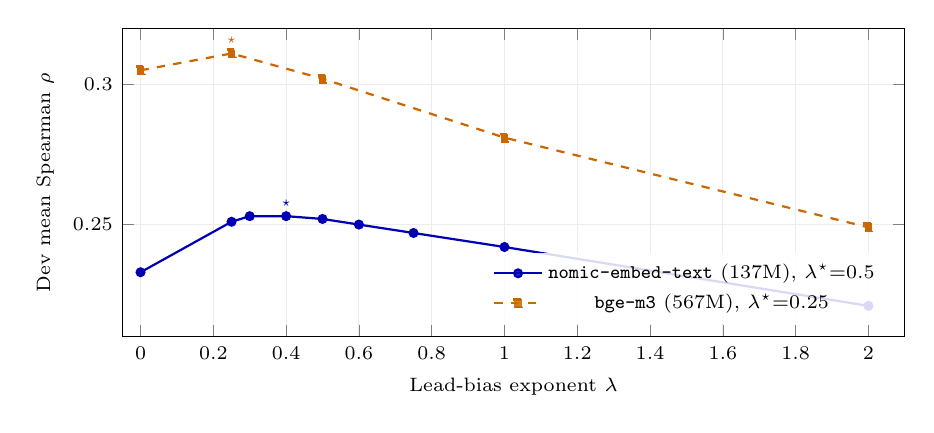
\begin{tikzpicture}
\begin{axis}[
  width=0.95\linewidth, height=5.5cm,
  xlabel={Lead-bias exponent $\lambda$},
  ylabel={Dev mean Spearman $\rho$},
  xmin=-0.05, xmax=2.1,
  ymin=0.21, ymax=0.32,
  grid=both, grid style={gray!15},
  legend style={font=\scriptsize, at={(0.98,0.04)}, anchor=south east,
                draw=none, fill=white, fill opacity=0.85,
                text opacity=1},
  tick label style={font=\scriptsize},
  label style={font=\scriptsize},
  every axis plot/.append style={mark size=1.4pt, line width=0.8pt}
]
\addplot[color=blue!70!black, mark=*] coordinates {
  (0.00, 0.233) (0.25, 0.251) (0.30, 0.253) (0.40, 0.253)
  (0.50, 0.252) (0.60, 0.250) (0.75, 0.247) (1.00, 0.242)
  (2.00, 0.221)
};
\addlegendentry{\texttt{nomic-embed-text} (137M), $\lambda^{\star}{=}0.5$}

\addplot[color=orange!80!black, mark=square*, dashed] coordinates {
  (0.00, 0.305) (0.25, 0.311) (0.50, 0.302) (1.00, 0.281)
  (2.00, 0.249)
};
\addlegendentry{\texttt{bge-m3} (567M), $\lambda^{\star}{=}0.25$}

% Mark the two optima
\node[font=\tiny, color=blue!70!black, above]  at (axis cs:0.40, 0.253) {$\star$};
\node[font=\tiny, color=orange!80!black, above] at (axis cs:0.25, 0.311) {$\star$};
\end{axis}
\end{tikzpicture}
\caption{Development-split mean Spearman $\rho$ across the four
\textsc{SummEval} dimensions as a function of the lead-bias
exponent $\lambda$, for the two sentence-embedder backbones whose
sweep is reported in this paper. Both curves peak at $\lambda>0$
and decline monotonically past the peak, but the position of the
peak \emph{shifts} between backbones (0.5 for
\texttt{nomic-embed-text}, 0.25 for \texttt{bge-m3}). Reusing the
nomic-tuned $\lambda{=}0.5$ with \texttt{bge-m3} would give
$\rho{=}0.302$, below its no-prior baseline of $0.305$. This is
the empirical motivation for treating the calibration protocol of
Section~\ref{sec:methodology} as an obligatory part of the method.}
\label{fig:lambda-curve}
\end{figure}

Figure~\ref{fig:lambda-perdim} decomposes the development-mean curve of
Figure~\ref{fig:lambda-curve} (\texttt{nomic-embed-text}) into
its four \textsc{SummEval} per-dimension components. The
decomposition shows that the $\lambda^{*}{=}0.5$ optimum is a
compromise: the four dimensions do not share a single $\lambda$
that is best for all of them. Coherence and relevance benefit
strongly from the prior --- coherence peaks broadly in the
$[0.25, 1.0]$ region, relevance continues to climb up to
$\lambda{=}2$ --- while consistency and fluency are best at the
\emph{lowest} non-zero $\lambda$ ($\lambda{=}0.25$) and
deteriorate sharply as $\lambda$ grows. The mean optimum at
$\lambda{=}0.5$ is the value that best balances the two pairs;
practitioners with a single dimension of interest may prefer a
different point on the curve.

\begin{figure}[t]
\centering
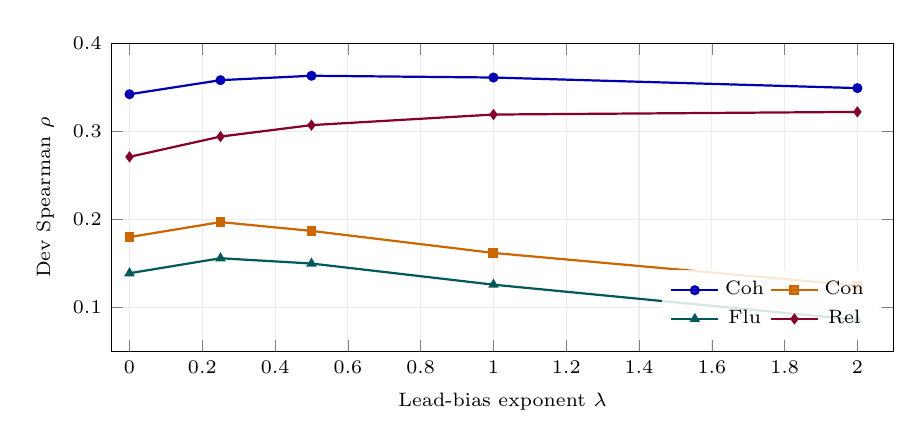
\begin{tikzpicture}
\begin{axis}[
  width=0.95\linewidth, height=5.5cm,
  xlabel={Lead-bias exponent $\lambda$},
  ylabel={Dev Spearman $\rho$},
  xmin=-0.05, xmax=2.1,
  ymin=0.05, ymax=0.40,
  grid=both, grid style={gray!15},
  legend style={font=\scriptsize, at={(0.98,0.04)}, anchor=south east,
                draw=none, fill=white, fill opacity=0.85,
                text opacity=1},
  legend columns=2,
  tick label style={font=\scriptsize},
  label style={font=\scriptsize},
  every axis plot/.append style={mark size=1.4pt, line width=0.8pt}
]
\addplot[color=blue!70!black, mark=*] coordinates {
  (0.00,0.342) (0.25,0.358) (0.50,0.363) (1.00,0.361) (2.00,0.349)
};
\addlegendentry{Coh}
\addplot[color=orange!80!black, mark=square*] coordinates {
  (0.00,0.180) (0.25,0.197) (0.50,0.187) (1.00,0.162) (2.00,0.125)
};
\addlegendentry{Con}
\addplot[color=teal!70!black, mark=triangle*] coordinates {
  (0.00,0.139) (0.25,0.156) (0.50,0.150) (1.00,0.126) (2.00,0.086)
};
\addlegendentry{Flu}
\addplot[color=purple!70!black, mark=diamond*] coordinates {
  (0.00,0.271) (0.25,0.294) (0.50,0.307) (1.00,0.319) (2.00,0.322)
};
\addlegendentry{Rel}
\end{axis}
\end{tikzpicture}
\caption{Per-dimension development-split Spearman $\rho$ versus the
lead-bias
exponent $\lambda$ with \texttt{nomic-embed-text}. Coherence and
relevance benefit from the prior across the swept range
($\lambda^{*}_{\text{Coh}}{=}0.5$,
$\lambda^{*}_{\text{Rel}}{=}2.0$); consistency and fluency peak
at the smallest non-zero value ($\lambda^{*}_{\text{Con}},
\lambda^{*}_{\text{Flu}}{=}0.25$) and degrade as $\lambda$ grows.
The canonical $\lambda^{*}{=}0.5$ is the optimum on the
mean-of-four criterion (Section~\ref{sec:methodology}), not on
any single dimension.}
\label{fig:lambda-perdim}
\end{figure}

\subsection{\texorpdfstring{How identifiable is $\lambda^{*}$?}{How identifiable is lambda*?}}
\label{sec:lambda-identifiability}
Every number reported so far treats $\lambda^{*}$ as if the
development split had determined it. It did not determine it; it
selected it, and a different draw of 50 articles would have selected
something else. Because the entire calibration protocol of
Section~\ref{sec:methodology} rests on that selection, we measure how
reproducible it is instead of assuming it.

The procedure is the cluster bootstrap of
Section~\ref{sec:methodology-bootstrap} applied one level up. On each
of $5{,}000$ resamples of the development articles we recompute the
mean Spearman $\rho$ at \emph{every} grid value and record which value
wins, yielding a distribution over the grid rather than a point.
Table~\ref{tab:lambda_selection_ci} reports it. Because the per-sample
scores for each $\lambda$ are already stored, the measurement requires
no additional embedder passes.

\begin{table*}[t]
\centering
\caption{Selection uncertainty of the lead-bias exponent. For each (split, backbone) the whole selection procedure --- compute mean Spearman $\rho$ across the four \textsc{SummEval} dimensions at every grid value, take the argmax --- is re-run on 5000 cluster-bootstrap resamples over articles. $P(\arg\max)$ is the fraction of resamples in which that grid value is selected; a selection procedure that identifies a well-separated optimum concentrates this mass on one row. $\lambda^{\star}$ marks the argmax of the point estimate, i.e.\ the value the ablation table reports.}
\label{tab:lambda_selection_ci}
\small
\linespread{1}\selectfont
\setlength{\tabcolsep}{4pt}
\begin{tabular}{@{}llrrr@{}}
\toprule
Split / backbone & $\lambda$ & Mean $\rho$ & 95\% CI & $P(\arg\max)$ \\
\midrule
dev / \texttt{bge-m3} & 0 & .305 & {\scriptsize [.248, .361]} & 13.8\% \\
 & 0.25 $\star$ & .311 & {\scriptsize [.254, .366]} & 84.2\% \\
 & 0.5 & .302 & {\scriptsize [.247, .355]} & 2.0\% \\
 & 1 & .281 & {\scriptsize [.231, .330]} & 0.0\% \\
 & 2 & .249 & {\scriptsize [.204, .295]} & 0.0\% \\
\addlinespace[3pt]
dev / \texttt{nomic-embed-text} & 0 & .233 & {\scriptsize [.168, .299]} & 0.7\% \\
 & 0.25 & .251 & {\scriptsize [.188, .315]} & 17.5\% \\
 & 0.3 & .253 & {\scriptsize [.189, .315]} & 27.6\% \\
 & 0.4 $\star$ & .253 & {\scriptsize [.189, .315]} & 20.4\% \\
 & 0.5 & .252 & {\scriptsize [.189, .314]} & 17.8\% \\
 & 0.6 & .250 & {\scriptsize [.188, .312]} & 9.9\% \\
 & 0.75 & .247 & {\scriptsize [.186, .308]} & 2.6\% \\
 & 1 & .242 & {\scriptsize [.182, .301]} & 2.9\% \\
 & 2 & .221 & {\scriptsize [.165, .276]} & 0.5\% \\
\addlinespace[3pt]
test / \texttt{nomic-embed-text} & 0 & .314 & {\scriptsize [.273, .352]} & 0.3\% \\
 & 0.25 $\star$ & .334 & {\scriptsize [.291, .371]} & 85.0\% \\
 & 0.3 & .332 & {\scriptsize [.289, .370]} & 14.6\% \\
 & 0.4 & .326 & {\scriptsize [.282, .365]} & 0.1\% \\
 & 0.5 & .319 & {\scriptsize [.274, .359]} & 0.0\% \\
 & 0.6 & .311 & {\scriptsize [.265, .352]} & 0.0\% \\
 & 0.75 & .299 & {\scriptsize [.252, .340]} & 0.0\% \\
 & 1 & .280 & {\scriptsize [.228, .325]} & 0.0\% \\
 & 2 & .237 & {\scriptsize [.182, .288]} & 0.0\% \\
\bottomrule
\end{tabular}
\vspace{2mm}
\begin{tabular}{@{}lrrr@{}}
\toprule
Paired comparison & $P(\lambda^{\star}_A{=}\lambda^{\star}_B)$ & $P(\lambda^{\star}_A{<}\lambda^{\star}_B)$ & $P(\lambda^{\star}_A{>}\lambda^{\star}_B)$ \\
\midrule
cross-backbone (shared draw) & 37.8\% & 0.4\% & 61.9\% \\
same backbone, two independent draws (noise floor) & 43.5\% & 28.6\% & 27.9\% \\
dev vs test, same backbone & 46.3\% & 0.9\% & 52.8\% \\
\bottomrule
\end{tabular}
\end{table*}


\paragraph{Switching the prior on is reproducible}
The no-prior setting $\lambda{=}0$ is selected in $0.7\%$ of
development resamples and $0.3\%$ of test resamples. Whatever else is
uncertain, the decision to impose \emph{some} positional prior is
not: it survives resampling in more than $99\%$ of draws on both
splits. This is the claim the ablation supports, and it is weaker
than --- and logically prior to --- any claim about a particular
exponent.

\paragraph{The exponent itself is not identifiable}
The selection mass does not concentrate. On the development split with
the canonical backbone, $\lambda{=}0.3$ wins $27.6\%$ of resamples,
$\lambda{=}0.4$ wins $20.4\%$, the reported $\lambda^{*}{=}0.5$ wins
$17.8\%$, and $\lambda{=}0.25$ wins $17.5\%$: four grid values within
ten points of each other, none commanding even a third of the mass.
A 50-article development split does not contain enough information to
separate them. The practical reading is that the protocol returns the
interval $[0.25, 0.6]$, inside which no value is distinguishable from
any other, and that quoting a three-significant-figure optimum from
such a surface overstates what was measured.

\paragraph{Two controls, and what they do to the backbone claim}
The lower panel of Table~\ref{tab:lambda_selection_ci} compares whole
selection outcomes rather than single $\rho$ values, on the grid
common to every configuration. The control that matters is the third
row of the reasoning: a configuration compared \emph{against itself}
on two independent draws of the same 50 articles reselects the same
exponent only $43.5\%$ of the time, and when it disagrees the
direction is a coin flip ($28.6\%$ versus $27.9\%$). That is the
noise floor. Against it, the cross-backbone agreement of $37.8\%$ is
barely lower --- so the observation that two backbones pick different
exponents is, on its own, uninformative.

What does separate from the noise floor is the \emph{direction}. When
\texttt{nomic-embed-text} and \texttt{bge-m3} are scored on the same
resample and disagree, the former selects the larger exponent in
$61.9\%$ of resamples against $0.4\%$ for the reverse, a ratio no
symmetric noise process produces. We therefore claim a directional
backbone effect --- \texttt{bge-m3} prefers a weaker prior --- and
explicitly do not claim a quantified shift from $0.5$ to $0.25$.

One confound must be stated because it limits even that claim. The
same asymmetry appears between the development and test splits under
an \emph{unchanged} backbone ($52.8\%$ versus $0.9\%$). Changing which
50 articles are used therefore induces a directional shift of
comparable strength to changing the representation space. Our design
cannot attribute the cross-backbone asymmetry to the backbone alone,
and a clean attribution would need the sweep repeated over many
disjoint article samples per backbone --- which, on a 100-article
benchmark, is not available. Section~\ref{sec:future-work} lists the
multi-corpus replication that would supply it.

\subsection{Backbone ablation}
\label{sec:ablation-embedder}
Table~\ref{tab:ablation_embedder} shows the canonical
$\lambda{=}0.5$ metric with four sentence-embedder backbones
spanning a $\sim$24$\times$ parameter range:
\texttt{all-minilm} (23M),
\texttt{nomic-embed-text} (137M),
\texttt{mxbai-embed-large} (335M), and
\texttt{bge-m3} (567M). The mean Spearman across the four
\textsc{SummEval} dimensions falls in $[.284, .312]$ for all four
backbones, a span of $.028$ across the full parameter range. We
read this as evidence that the metric \emph{design}
--- the mean-of-max grounding aggregator with the lead-bias prior
--- is qualitatively robust to backbone choice: any reasonable
sentence embedder produces a working metric.

Two properties of this table need to be stated explicitly, because
both cut against the headline numbers rather than for them. First,
\texttt{nomic-embed-text} --- the canonical backbone, fixed before
the ablation was run --- has the \emph{lowest} mean of the four
(.284, against .296 for \texttt{mxbai-embed-large}, .298 for
\texttt{all-minilm} and .312 for \texttt{bge-m3}). The headline
correlations of Tables~\ref{tab:correlations_summary} and
\ref{tab:compare_lgs_summary}, and the Pareto position of
Section~\ref{sec:pareto}, are therefore reported at the conservative
end of the observed band; a backbone swap to \texttt{bge-m3} would
raise the mean $\rho$ to .312 without changing the design, at roughly
$5\times$ the embedding cost. We keep the pre-registered canonical
backbone rather than the best-performing one, because selecting the
backbone on the same data used for the headline table would be a
researcher degree of freedom we would rather not exercise.

Second, the per-dimension profile is not stable across backbones.
\texttt{nomic-embed-text} is by far the strongest on
coherence (.396) and relevance (.356) and the weakest on consistency
(.227) and fluency (.156); the other three backbones invert this
pattern. \emph{Per-dimension} comparisons against baselines --- for
instance, ``LGS exceeds BERTScore on consistency'' --- are therefore
valid for the specific backbone used and should be read as
backbone-conditional, not as universal properties of LGS. The
mean-Spearman ordering of metric families is stable across backbones;
the per-dimension ordering is not.

\input{embedders.gen.tex}

\subsection{Cross-backbone calibration of the prior}
\label{sec:ablation-lead-bge}
The backbone ablation also bears on \emph{where} the prior should be
set, not only on how well the metric scores.
Figure~\ref{fig:lambda-curve} shows the development-split mean Spearman
$\rho$ as a function of $\lambda$ for two embedders:
\texttt{nomic-embed-text} (the canonical backbone) and
\texttt{bge-m3} (the largest in our roster, chosen as the
strongest contrast point). Both curves share their qualitative
shape: each peaks at $\lambda{>}0$ --- that is, the injected
structural knowledge helps regardless of the backbone --- and declines
monotonically past the peak. But the position of the peak
\emph{shifts}: $\lambda^{*}{=}0.5$ for \texttt{nomic-embed-text}
(development mean $.252$, a lift of $+.019$ over the no-prior
baseline) and $\lambda^{*}{=}0.25$ for \texttt{bge-m3}
(development mean $.311$, a lift of only $+.006$).

The practical consequence is sharp: applying the nomic-tuned
$\lambda{=}0.5$ to \texttt{bge-m3} yields a development mean of $.302$,
which is \emph{below} its no-prior baseline of $.305$. A prior that
helps when its exponent is calibrated against the backbone in use can
therefore cost more than it returns when an exponent is carried over
from elsewhere.

Two qualifications are essential, and
Section~\ref{sec:lambda-identifiability} supplies both. First, the gap
between $.302$ and $.305$ is a fraction of the bootstrap half-width,
so this particular pair of numbers is an illustration rather than a
demonstration. What carries statistical weight is the directional
result: scored on the same resample, \texttt{nomic-embed-text} selects
the larger exponent $61.9\%$ of the time against $0.4\%$ for the
reverse. Second, that asymmetry is not uniquely attributable to the
backbone, because a change of article sample under a fixed backbone
produces one of comparable strength. The defensible claim is therefore
that the exponent should be re-derived in situ --- not that the
backbone is the specific variable that invalidates a borrowed value.
That weaker claim is sufficient for the protocol, since the sweep is
what transfers and it costs no additional embedder passes.

We hypothesise that the size of the lift depends on the density of the
backbone's representation. \texttt{bge-m3} already produces a
stronger position-agnostic recall (.305 development mean at
$\lambda{=}0$, versus $.233$ for \texttt{nomic-embed-text}), leaving
less room for a positional prior to add value. We flag this as a
hypothesis rather than a result: with two backbones swept and an
exponent that Section~\ref{sec:lambda-identifiability} shows to be
poorly identified, the evidence does not discriminate between it and
simpler accounts. The general lesson we do draw is weaker and, we
think, more durable: an a priori structural prior and a learned
representation are not independent components, and how much the
explicit prior can still contribute is not knowable without
measurement on the deployment's own data.

% ------------------------------------------------------------------
\section{Discussion}
\label{sec:discussion}

\subsection{Decision-support deployment scenarios}
\label{sec:deployment}
LGS is designed for three decision procedures that reference-based
and LLM-judge metrics serve poorly. The first is \emph{online
model selection}: a summarisation system serves many candidates
per source article (multiple decoding configurations, multiple
prompt variants, multiple checkpoints under A/B test), and the
operator needs a low-latency, deterministic score to pick the
best candidate per request. Reference-based metrics are
unavailable because there is no human reference for production
inputs; G-Eval's per-candidate judge call is too expensive
and its sampled decoding too non-deterministic to make ranking
reproducible across replays. LGS is reference-free, deterministic
up to the embedder's numerical precision, and adds approximately
one CPU sentence-embedder forward pass per source and per
candidate sentence to the request budget --- with the source side
amortised across candidates
(Section~\ref{sec:complexity}).

The second is \emph{automated release gating}. A
continuous-integration pipeline replays a fixed
corpus of source articles through both the previous and
candidate model versions and blocks a merge on a significant
regression. Such
pipelines run at high frequency (per commit, per nightly
build) over many thousands of articles; the cost of a judge
or fine-tuned-encoder pass per (article, candidate) pair under
this load is prohibitive. The reference-free, embedding-only
profile of LGS makes the wall-clock overhead negligible, and
its single hyperparameter is fixed at deployment time, so the
score is a stable signal across runs. Determinism matters here
beyond cost: a gate that fires non-deterministically is not a gate.

The third is \emph{reward modelling for reinforcement-learning
fine-tuning of summarisation systems}. Such training generates many
candidates per article per step, requiring a fast and stable reward
signal. LGS produces a deterministic scalar per candidate from a
single embedder pass, which is compatible with the iteration speed
demanded by these training loops, and the source-side embedding cache
is reused across the whole rollout for a given article. We do not
claim that LGS is the ideal reward signal --- specialised reward
models tuned to the target dimension would likely dominate --- but it
is a viable default when no such specialised model exists,
particularly on news-domain corpora where the injected prior matches
the underlying distribution.

In all three cases the metric is consumed by an automated procedure
that must justify its decision to a human afterwards. The argmax
anchors of Algorithm~\ref{alg:lgs} serve that purpose: a rejected
candidate can be reported together with the specific summary
sentences that failed to find support in the source and the source
sentences that came closest, which neither a whole-text cosine nor a
judge's numeric verdict provides without extra work.

\subsection{What LGS does and does not claim}
We make four claims and explicitly disclaim the stronger versions of
each.
(i)~Among the thirteen published, non-trivial baselines in our
controlled benchmark, LGS occupies an undominated cost--quality point
and strictly dominates six widely used metrics. We do \emph{not} claim
Pareto-optimality against the full pool: once reference-free
lead-window controls are included, LGS is strictly dominated on the
raw mean-correlation axis (Section~\ref{sec:pareto}), and on the
confound-controlled axis it is not statistically distinguishable from
the cheapest such control (Section~\ref{sec:confound-analysis}). Nor
do we claim the highest correlation --- UniEval is higher on every
dimension and we report that directly.
(ii)~The injected lead-bias prior produces a held-out lift on the
\emph{mean} Spearman $\rho$ across the four \textsc{SummEval}
dimensions and on \emph{coherence} specifically; we do
\emph{not} claim a held-out per-dimension lift on consistency,
fluency, or relevance, where the development-side improvements
($+.007$, $+.011$, $+.036$ respectively) attenuate to within
bootstrap noise on test ($-.001$, $+.001$, $+.003$).
(iii)~Imposing some positional prior is supported: $\lambda{=}0$ is
selected in under $1\%$ of bootstrap resamples on either split. We do
\emph{not} claim that $\lambda^{*} = 0.5$ is the optimum, universal or
otherwise --- it wins $17.8\%$ of development resamples, three other
grid values win comparable shares, and an unchanged configuration
reselects it only $43.5\%$ of the time across two draws. What the
protocol returns is the interval $[0.25, 0.6]$
(Section~\ref{sec:lambda-identifiability}). We further claim a
\emph{directional} backbone effect --- \texttt{bge-m3} prefers a
weaker prior --- but not a quantified shift, and we note that a change
of article sample under a fixed backbone produces a directional shift
of comparable strength, so the backbone is not isolated as the cause
(Section~\ref{sec:ablation-lead-bge}).
(iv)~The cost figures characterise a single-machine, CPU-only,
single-thread deployment target; we do \emph{not} claim that the same
ratios hold under GPU serving or batched inference, although the
structural difference between one small embedder pass and $N$
autoregressive decodes is not a property of the hardware.

\subsection{Practitioner recommendations}
\label{sec:practitioner}
For readers considering LGS as a deployed metric, the empirical
findings above translate into four operational
recommendations. First, \emph{run the calibration sweep}. The optimal
$\lambda$ depends on the backbone
(Section~\ref{sec:ablation-lead-bge}), and reusing a published
$\lambda$ value from a different backbone can degrade the metric
below its no-prior baseline. The sweep is cheap --- five
$\lambda$ values on a 50-article development split take
approximately five minutes on the canonical
\texttt{nomic-embed-text} backbone, and require no additional
embedder passes beyond the first
(Section~\ref{sec:complexity}) --- and is the operational
price of an explicit structural prior.
Second, \emph{decide whether the mean or a single dimension is
the deployment target}. The canonical $\lambda^{*}{=}0.5$
optimises the mean across the four \textsc{SummEval} dimensions;
if the deployment cares specifically about coherence or relevance
the optimum shifts toward larger $\lambda$, and if it cares
about consistency or fluency the optimum shifts toward the
smallest non-zero $\lambda$ in the grid
(Figure~\ref{fig:lambda-perdim}).
Third, \emph{pick the backbone on the deployment's cost budget, not
on ours}. The backbone ablation
(Section~\ref{sec:ablation-embedder}) shows the mean $\rho$ varies by
only $.028$ across a $24\times$ parameter range, so a deployment that
can afford \texttt{bge-m3} gains a slightly higher mean, and one that
cannot loses very little by using a 23M-parameter embedder --- but the
per-dimension profile changes substantially, so the choice should be
made against the dimension that matters.
Fourth, \emph{re-tune $\lambda$ when migrating backbones}. A
backbone change is not a drop-in replacement; it is a new
deployment from the metric's perspective.

\subsection{Limitations}
\label{sec:limitations}
\textit{Domain.} \textsc{SummEval} contains only CNN/DailyMail news
articles. Lead bias is a well-documented structural property of
this corpus, and LGS exploits it explicitly through the
exponential prior. Domains without a strong leading-sentence
structure --- scientific abstracting, narrative or dialogue
summarisation, long-form question answering --- may require a
different prior or none at all. We do not claim that the
exponential lead-bias formulation transfers; we claim that the
\emph{protocol} of selecting and calibrating a structural source-side
prior on a held-out split transfers, and that the prior shape
itself is a domain-specific design choice.

\textit{G-Eval baseline configuration.} Our G-Eval baseline uses
$N\!=\!3$ independent runs at temperature $0.7$ with
\texttt{qwen2.5:7b-instruct-q4\_K\_M} and reports the across-run
mean as the canonical score. The original paper averages 20
GPT-4 samples; our setup is therefore a budget reproduction.
The across-run standard deviation of summary-level Spearman is
between $.003$ and $.009$ across the four dimensions, well below
the half-width of the paired-bootstrap confidence intervals, so
judge stochasticity is not a meaningful confound for the
LGS-vs-G-Eval comparisons. We document this explicitly because
single-run G-Eval baselines in the literature do not.

\textit{Prior shape.} The lead-bias prior is exponential. Linear,
reciprocal, and hard-cutoff alternatives have not been tested;
we leave them as future work (Section~\ref{sec:future-work}).

\textit{Backbone.} The headline numbers use
\texttt{nomic-embed-text} with $\lambda^*$ calibrated against it. The
ablation in Section~\ref{sec:ablation-embedder} shows
that mean Spearman is qualitatively stable across a $\sim24\times$
parameter range, but per-dimension profiles shift; numbers
quoted at the per-dimension granularity should be read as
backbone-conditional.

\subsection{Threats to validity}
\label{sec:threats}
We flag four threats to the validity of the conclusions drawn in
this paper that a careful reader should weigh.

\textit{Single-corpus evidence.} All correlation numbers are
computed on \textsc{SummEval}, a single benchmark
derived from a single news corpus (CNN/DailyMail). The
\emph{methodological} contributions --- the article-level
held-out split, the cluster-bootstrap discipline, the cost-controlled
protocol, and the demonstration that the optimal exponent
shifts across backbones --- are corpus-independent in principle,
but the \emph{numerical} headline correlations transfer to other
corpora only to the degree that those corpora share the
lead-bias structural property of \textsc{SummEval} articles. We
consider a multi-corpus replication the single most valuable
extension of this work (Section~\ref{sec:future-work}).

\textit{Reproductions versus original-paper numbers.} As discussed
in Section~\ref{sec:experiments} and
Table~\ref{tab:simplifications}, our baseline numbers are not the
original-paper numbers. They are reproductions under
budget-feasible configurations on a single laptop-scale
deployment target, which is what makes the cost axis meaningful.
Cross-paper number comparisons should therefore be made against the
original references, not against our reproductions; our reproductions
are internally self-consistent for the cross-baseline comparisons we
report, and the Pareto structure of Section~\ref{sec:pareto} is a
statement about this internally consistent pool.

\textit{Stochasticity of the LLM judge.} Our G-Eval
configuration uses $N{=}3$ samples at temperature 0.7. The
across-run standard deviation of summary-level Spearman is
between $.003$ and $.009$, which we have argued is small enough
not to be a meaningful confound for the LGS-vs-G-Eval comparisons
(Section~\ref{sec:limitations}). A full $N{=}20$ reproduction at
temperature 1 with a frontier-grade judge would shrink this
further and would raise G-Eval's correlation, but at a
proportionally higher cost, so it would not move G-Eval onto the
Pareto frontier unless the correlation gain exceeded UniEval's.

\textit{Backbone calibration of the score scale.} The cosine
similarity values used inside LGS are not calibrated probabilities;
they are raw inner products in a learned representation space. The
metric is therefore meaningful as a \emph{ranker} of summaries (which
is what Spearman measures) but should not be interpreted as a
calibrated quality score on an absolute scale.

\subsection{Future work}
\label{sec:future-work}
Four directions extend the current contribution most directly.
First, transfer to non-news corpora, which is where the injected
knowledge is most at risk: scientific abstracting
(\textsc{ArXiv}, \textsc{PubMed}, see~\cite{cohan2018arxiv})
and dialogue summarisation
(\textsc{SAMSum}~\cite{gliwa2019samsum}, \textsc{DialogSum}) are
natural next benchmarks, and the prior shape is the variable we
expect to re-tune --- or to remove, if the corpus has no positional
salience structure.
Second, alternative shapes for the source-position prior: linear
$w(i)=\max(0, 1-\lambda i/n)$, reciprocal
$w(i)=1/(1+\lambda i/n)$, and a hard cutoff at the first $k$
sentences. The calibration protocol of
Section~\ref{sec:methodology} applies unchanged.
Third, richer sources of structural knowledge than position:
salience weighting derived from discourse parsing, section headings
in structured documents, or entity-centrality signals over the source
--- all of which fit the same multiplicative source-side slot as
$w(i)$ and can be ablated the same way.
Fourth, alternative aggregation operators on the candidate side:
low-percentile recall (a hallucination-sensitive variant) and
position-weighted top-$k$ recall, evaluated against the diffusion
pattern documented in Appendix~\ref{app:extension-log}.

% ------------------------------------------------------------------
\section{Conclusion}
\label{sec:conclusion}

We presented LGS, a reference-free, embedding-only operator for
summary quality assessment, defined as
$\mathrm{LGS}(D,C){=}\mathrm{mean}_j \max_i\, w(i)\cos(c_j, s_i)$
with an exponential lead-bias prior $w(i){=}\exp(-\lambda i / n)$
over source-sentence position. The prior is the point of the design:
it injects one explicit, auditable piece of discourse-structural
domain knowledge into a subsymbolic similarity space, at zero
inference cost and with a single interpretable parameter that can be
set to zero to remove it exactly.

Measured against thirteen published baselines on \textsc{SummEval}
under one controlled hardware budget, LGS occupies an undominated
cost--quality point and strictly dominates six widely used metrics
--- among them BERTScore, whose mean summary-level Spearman $\rho$ it
exceeds while running roughly ten times faster and without access to
the human reference summary. In the same analysis the LLM-judge
baseline is itself dominated by the fine-tuned-encoder baseline --- a
statement about the budget configurations of
Table~\ref{tab:simplifications}, not about G-Eval with a
frontier-grade judge, and one we make only for the reproduction pool
defined in Section~\ref{sec:experiments}.

That result does not survive the control a reviewer of an earlier
version of this paper correctly demanded: a trivial reference-free
lead-window heuristic, at roughly three orders of magnitude lower
cost, matches or beats LGS's own raw mean correlation
(Section~\ref{sec:pareto}). We traced this to a confound in the
benchmark itself --- \textsc{SummEval}'s human ratings substantially
reward verbatim copying from the source, and a parameter-free copy-rate
counter alone outranks eleven of the fourteen published metrics in our
pool (Section~\ref{sec:confound-analysis}). Once that confound is
controlled for, LGS is no longer statistically distinguishable from
the cheapest lead-window control, and it ties rather than beats
BERTScore. We regard this as the central limitation of the paper: the
sentence-level grounding mechanism LGS is built around does not
demonstrably contribute more than a four-line lexical heuristic once
the benchmark's extractiveness confound is removed, and we report that
finding in full rather than reframing the metric pool to obscure it.
We are explicit that UniEval attains a higher correlation than LGS on
every dimension regardless of which axis is used; the claim of this
paper, appropriately narrowed, is an undominated position among
learned and embedding-based metrics, not a correlation record and not
an unqualified Pareto-optimality claim.

The second contribution is methodological and, we believe, transfers
beyond this metric. Submitting the hyperparameter \emph{selection
procedure} to the same bootstrap that validates the correlations
separates two claims that a point estimate conflates. That the prior
should be switched on is reproducible: the no-prior setting is
selected in under $1\%$ of resamples. Which exponent to switch it to
is not: the reported value wins under a fifth of resamples, and an
unchanged configuration reselects it less than half the time across
two draws of the same articles. A knowledge-informed metric of this
kind should therefore be published as a \emph{design plus an
obligatory calibration protocol} that returns an interval, not as a
fixed numerical recipe --- and the width of that interval belongs in
the paper, because a practitioner who copies a published exponent is
otherwise copying one draw's answer to an underdetermined question.
The calibration is cheap --- five $\lambda$ values on 50 articles,
approximately five minutes on a laptop CPU thread, with no additional
embedder passes --- and the cost of skipping it is silent
miscalibration. The same discipline applies to alternative priors and
alternative aggregation operators; Appendix~\ref{app:extension-log}
records the components we tested and rejected, together with the
structural pattern extracted from those negative results.

% ------------------------------------------------------------------
\section*{Reproducibility}
\label{sec:repro}
The full pipeline is open-source and deterministic up to the
sentence embedder's numerical precision. The repository
(\url{https://github.com/mikolajsemeniuk/llmbench}) contains a
\texttt{Makefile} reproducing every table and figure in this
paper end-to-end: \texttt{make benchmark} runs all 14 metrics on
\textsc{SummEval}, \texttt{make benchmark-ablation} runs the
$\lambda$ sweep on the development and test splits,
\texttt{make benchmark-embedder-ablation} runs the canonical
metric with the four backbones, and \texttt{make paper}
regenerates every \texttt{.tex} table from the corresponding
JSON outputs. The selection-uncertainty analysis of
Section~\ref{sec:lambda-identifiability} is
\texttt{make paper-lambdaci}, and the multiple-comparison correction
of Section~\ref{sec:methodology-bootstrap} is applied inside
\texttt{cmd/compare}; both read the stored per-sample scores and
need neither Ollama nor the model server, so a reviewer can
reproduce every statistical claim in this paper without running a
single metric. Bootstrap seeds are fixed in \texttt{pkg/eval}
(seed 42 for cluster bootstrap, seed-derived for paired
comparisons). The sentence embedders are pinned by Ollama tag in
the Makefile (\texttt{nomic-embed-text},
\texttt{mxbai-embed-large}, \texttt{bge-m3}, \texttt{all-minilm});
the G-Eval judge is \texttt{qwen2.5:7b-instruct-q4\_K\_M}
under the same Ollama runtime. \textsc{SummEval} itself is
publicly available under the original authors'
release~\cite{fabbri2021summeval}; the JSONL split used for the
article-level development/test partition is the SummEval canonical
release order, deterministic without a random seed.

% ------------------------------------------------------------------
\section*{CRediT authorship contribution statement}
\textbf{Mikolaj Semeniuk:} Conceptualization, Methodology, Software,
Validation, Formal analysis, Investigation, Data curation,
Visualization, Writing -- original draft.
\textbf{Agnieszka Jastrzebska:} Conceptualization, Methodology,
Validation, Supervision, Project administration, Writing -- review
\& editing.

\section*{Declaration of competing interest}
The authors declare that they have no known competing financial
interests or personal relationships that could have appeared to
influence the work reported in this paper.

\section*{Funding}
This research did not receive any specific grant from funding
agencies in the public, commercial, or not-for-profit sectors.

\section*{Data availability}
All data and code required to reproduce every result in this paper
are publicly available. The source code, the reproduction
\texttt{Makefile}, and the per-sample score files for all fourteen
metrics are released at
\url{https://github.com/mikolajsemeniuk/llmbench}. The
\textsc{SummEval} benchmark is publicly distributed by its original
authors~\cite{fabbri2021summeval}.

\section*{Declaration of generative AI and AI-assisted technologies in the writing process}
During the preparation of this work the authors used a
generative AI assistant in order to improve the language and
readability of the manuscript. After using this tool, the authors
reviewed and edited the content as needed and take full
responsibility for the content of the published article.

% ------------------------------------------------------------------
\appendix

\section{Kendall $\tau$ Correlations}
\label{app:kendall}
Section~\ref{sec:methodology-corr} states that Spearman $\rho$ is the
primary correlation coefficient of this study and Kendall $\tau$ a
secondary check. Tables~\ref{tab:correlations_summary_kendall} and
\ref{tab:correlations_system_kendall} report the $\tau$ counterparts of
Tables~\ref{tab:correlations_summary} and
\ref{tab:correlations_system}, with the same article-level cluster
bootstrap. The two coefficients induce almost the same ordering of the
fourteen metrics --- the rank correlation between the $\rho$-ordering
and the $\tau$-ordering is $.996$ on coherence, $1.000$ on
consistency, $.987$ on fluency and $.996$ on relevance, and no metric
changes rank by more than two positions on any dimension. The
conclusions of Section~\ref{sec:results} are therefore invariant to the
choice between the two rank coefficients.

\begin{table*}[t]
\centering
\caption{Summary-level correlations with human judgment on SummEval. $\tau$ = Kendall. Brackets give the 95\% cluster-bootstrap confidence interval over articles.}
\label{tab:correlations_summary_kendall}
\small
\linespread{1}\selectfont
\setlength{\tabcolsep}{4pt}
\begin{tabular}{@{}lrrrr@{}}
\toprule
Metric & \multicolumn{1}{c}{Coh} & \multicolumn{1}{c}{Con} & \multicolumn{1}{c}{Flu} & \multicolumn{1}{c}{Rel} \\
\midrule
BLEU & .072 {\scriptsize [.024, .115]} & .107 {\scriptsize [.065, .147]} & .051 {\scriptsize [.005, .097]} & .148 {\scriptsize [.094, .203]} \\
ROUGE-L & .115 {\scriptsize [.067, .162]} & .110 {\scriptsize [.062, .154]} & .083 {\scriptsize [.036, .134]} & .144 {\scriptsize [.084, .202]} \\
ChrF & .112 {\scriptsize [.065, .160]} & .137 {\scriptsize [.101, .174]} & .086 {\scriptsize [.043, .132]} & .210 {\scriptsize [.158, .264]} \\
METEOR & .139 {\scriptsize [.100, .176]} & .105 {\scriptsize [.064, .143]} & .101 {\scriptsize [.051, .151]} & .131 {\scriptsize [.078, .179]} \\
SMART-String & -.004 {\scriptsize [-.051, .043]} & .087 {\scriptsize [.043, .130]} & .081 {\scriptsize [.037, .123]} & .088 {\scriptsize [.034, .143]} \\
EmbedScorer & .197 {\scriptsize [.153, .238]} & .044 {\scriptsize [-.004, .088]} & .031 {\scriptsize [-.018, .081]} & .229 {\scriptsize [.179, .279]} \\
BERTScore & .269 {\scriptsize [.225, .307]} & .085 {\scriptsize [.038, .128]} & .110 {\scriptsize [.063, .156]} & .270 {\scriptsize [.224, .318]} \\
MoverScore & .106 {\scriptsize [.059, .150]} & -.020 {\scriptsize [-.066, .026]} & .009 {\scriptsize [-.045, .057]} & .072 {\scriptsize [.016, .125]} \\
SMART-Model & .233 {\scriptsize [.191, .273]} & .074 {\scriptsize [.029, .116]} & .052 {\scriptsize [.004, .103]} & .229 {\scriptsize [.182, .277]} \\
BARTScore & .117 {\scriptsize [.075, .161]} & .092 {\scriptsize [.046, .137]} & .083 {\scriptsize [.033, .132]} & .195 {\scriptsize [.141, .252]} \\
GPTScore & .256 {\scriptsize [.218, .293]} & .166 {\scriptsize [.119, .216]} & .142 {\scriptsize [.096, .194]} & .221 {\scriptsize [.175, .264]} \\
UniEval & .408 {\scriptsize [.378, .437]} & .323 {\scriptsize [.293, .353]} & .352 {\scriptsize [.317, .385]} & .334 {\scriptsize [.293, .370]} \\
G-Eval & .318 {\scriptsize [.276, .361]} & .448 {\scriptsize [.410, .484]} & .131 {\scriptsize [.094, .165]} & .345 {\scriptsize [.293, .398]} \\
LGS & .285 {\scriptsize [.243, .326]} & .179 {\scriptsize [.137, .219]} & .120 {\scriptsize [.076, .169]} & .257 {\scriptsize [.216, .298]} \\
\bottomrule
\end{tabular}
\end{table*}

\begin{table*}[t]
\centering
\caption{System-level correlations with human judgment on SummEval. $\tau$ = Kendall. Brackets give the 95\% cluster-bootstrap confidence interval over articles.}
\label{tab:correlations_system_kendall}
\small
\linespread{1}\selectfont
\setlength{\tabcolsep}{4pt}
\begin{tabular}{@{}lrrrr@{}}
\toprule
Metric & \multicolumn{1}{c}{Coh} & \multicolumn{1}{c}{Con} & \multicolumn{1}{c}{Flu} & \multicolumn{1}{c}{Rel} \\
\midrule
BLEU & .183 {\scriptsize [-.276, .607]} & .017 {\scriptsize [-.407, .459]} & .283 {\scriptsize [-.228, .691]} & .350 {\scriptsize [-.146, .709]} \\
ROUGE-L & .217 {\scriptsize [-.243, .636]} & -.017 {\scriptsize [-.477, .424]} & .250 {\scriptsize [-.183, .648]} & .317 {\scriptsize [-.143, .712]} \\
ChrF & .350 {\scriptsize [-.045, .673]} & .617 {\scriptsize [.351, .852]} & .617 {\scriptsize [.357, .835]} & .617 {\scriptsize [.375, .804]} \\
METEOR & .000 {\scriptsize [-.472, .404]} & -.200 {\scriptsize [-.568, .264]} & .033 {\scriptsize [-.439, .523]} & .067 {\scriptsize [-.439, .486]} \\
SMART-String & -.150 {\scriptsize [-.655, .297]} & -.117 {\scriptsize [-.469, .268]} & .117 {\scriptsize [-.299, .535]} & .150 {\scriptsize [-.386, .593]} \\
EmbedScorer & .350 {\scriptsize [.009, .646]} & .283 {\scriptsize [-.091, .630]} & .183 {\scriptsize [-.232, .540]} & .217 {\scriptsize [-.171, .596]} \\
BERTScore & .617 {\scriptsize [.254, .887]} & -.017 {\scriptsize [-.473, .460]} & .250 {\scriptsize [-.232, .702]} & .383 {\scriptsize [-.086, .796]} \\
MoverScore & .083 {\scriptsize [-.416, .541]} & -.450 {\scriptsize [-.764, -.045]} & -.283 {\scriptsize [-.707, .174]} & -.150 {\scriptsize [-.655, .345]} \\
SMART-Model & .533 {\scriptsize [.164, .802]} & .467 {\scriptsize [.055, .790]} & .400 {\scriptsize [-.089, .784]} & .467 {\scriptsize [-.027, .874]} \\
BARTScore & .367 {\scriptsize [-.064, .694]} & .633 {\scriptsize [.382, .870]} & .567 {\scriptsize [.315, .784]} & .600 {\scriptsize [.327, .835]} \\
GPTScore & .500 {\scriptsize [.053, .842]} & .400 {\scriptsize [-.018, .762]} & .300 {\scriptsize [-.236, .770]} & .367 {\scriptsize [-.141, .852]} \\
UniEval & .650 {\scriptsize [.298, .911]} & .367 {\scriptsize [-.057, .750]} & .583 {\scriptsize [.252, .836]} & .633 {\scriptsize [.321, .844]} \\
G-Eval & .400 {\scriptsize [-.018, .752]} & .745 {\scriptsize [.491, .909]} & .226 {\scriptsize [-.271, .661]} & .650 {\scriptsize [.256, .927]} \\
LGS & .467 {\scriptsize [.009, .892]} & .467 {\scriptsize [.135, .735]} & .400 {\scriptsize [-.088, .807]} & .433 {\scriptsize [-.035, .861]} \\
\bottomrule
\end{tabular}
\end{table*}


\section{Extension Log: Components Tested and Rejected}
\label{app:extension-log}
The canonical LGS reported in this paper has a single tunable
hyperparameter, $\lambda$. This minimal design is the result of a
sequence of ablations conducted during calibration;
each rejected component below was tested under the same held-out
protocol of Section~\ref{sec:methodology} (sweep on the
50-article development split, mean Spearman $\rho$ across the
four \textsc{SummEval} dimensions as the selection criterion,
verification on the 50-article test split). We document them
here so that readers can see what was tried, why it was rejected,
and what general lesson the rejection encoded.

Table~\ref{tab:extension-log} summarises the development-split mean
Spearman
$\rho$ at the optimum of each rejected component's grid, against
the no-prior recall baseline ($\rho{=}.233$) and the accepted
lead-bias prior ($\rho{=}.252$ at $\lambda^{*}{=}0.5$).

\begin{table*}[!ht]
\centering
\caption{LGS components tested during calibration. Development-split
mean Spearman $\rho$ averaged across the four \textsc{SummEval}
dimensions on the 50-article development split. Only the
lead-bias prior was retained in the canonical metric.}
\label{tab:extension-log}
\footnotesize
\setlength{\tabcolsep}{4pt}
\begin{tabular}{@{}p{0.14\linewidth} p{0.38\linewidth} p{0.16\linewidth} p{0.26\linewidth}@{}}
\toprule
\textbf{Component} & \textbf{Form} & \textbf{Dev $\rho$ at optimum} & \textbf{Verdict} \\
\midrule
Recall baseline             & $\mathrm{mean}_j \max_i \cos(c_j, s_i)$
                            & .233 & reference point. \\
Lead-bias prior $\lambda$   & $\mathrm{mean}_j \max_i w(i)\cos(c_j, s_i)$, $w(i){=}\exp(-\lambda i/n)$
                            & \textbf{.252} ($\lambda^{*}{=}0.5$) & \textbf{accepted}: only component to lift the development mean over the baseline. \\
Legacy F$_{\beta}$ precision & $F_{\beta}(R, P)$ with $P$ over top-$30\%$ source by degree centrality
                            & .228 ($\beta{=}2$, frac${=}.30$) & rejected: aids relevance only by ${\sim}{+}.02$, loses 3/4 dimensions. \\
Anchor coverage $C^{\alpha}$ & $R \cdot C^{\alpha}$, $C{=}|\text{distinct argmax}_i|/m$
                            & .229 ($\alpha{=}.25$) & rejected: optimum at $\alpha{=}0$ (no coverage). \\
Within-summary diversity $D^{\gamma}$ & $R \cdot D^{\gamma}$, $D{=}1{-}\text{mean}_{j<k}\cos(c_j, c_k)$
                            & .209 ($\gamma{=}.10$) & rejected: monotonically harmful for $\gamma{>}0$. \\
Top-$k$ recall              & $\mathrm{mean}_j \tfrac{1}{k}\sum_{\text{top-}k} \cos(c_j, s_i)$
                            & .213 ($k{=}2$) & rejected: monotonically harmful for $k{>}1$. \\
\bottomrule
\end{tabular}
\end{table*}

\paragraph{Pattern across rejections}
Three of the four rejected components --- coverage, top-$k$
recall, and within-summary diversity --- share a structural
feature: each multiplies the recall term by a value in $[0, 1]$
that \emph{diffuses} the matching signal across multiple
candidate--source pairings. The empirical pattern is consistent:
each diffusion-style component improves relevance marginally
while degrading coherence, consistency, and fluency more than it
helps. We interpret this as evidence that a sharply localised
candidate-to-source grounding (single best match, no penalty) is
the strongest signal for \textsc{SummEval} on three of four
dimensions, and that modifications which disperse this
localisation hurt overall correlation.

The accepted component (the lead-bias prior) does \emph{not}
diffuse. It is a source-side structural prior that concentrates
weight on high-information positions \emph{before} the argmax,
without spreading the candidate-side aggregation. This is
consistent with the diffusion hypothesis: priors that reshape
the source without spreading the candidate-side aggregator are
the operations most likely to help.

\paragraph{Implication for future variants}
Future extensions of LGS proposed under the same protocol
should be evaluated against this pattern. A new component that
multiplies recall by a candidate-side coverage or diversity term
is unlikely to lift the development mean unless its formulation
specifically avoids the diffusion problem documented here.
Source-side priors (alternative decay shapes, salience-based
weighting, structural weighting derived from discourse parsing) are
the higher-prior direction for future work; we list specific
candidates in Section~\ref{sec:future-work}.

%\clearpage
% ------------------------------------------------------------------
\bibliographystyle{elsarticle-num}
\bibliography{references}

\end{document}
